\newpage
\def\tenchude{HỆ THỨC LƯỢNG TRONG TAM GIÁC}
\setcounter{dang}{0}
\setcounter{section}{5}
\section{Hệ thức lượng trong tam giác}
\subsection{KIẾN THỨC TRỌNG TÂM}
\subsubsection{Định lý cosin}
\begin{khung4}{}
	\immini{ Cho tam giác $ ABC$ có $ BC=a$, $ AC=b$ và $ AB=c$.
		\begin{itemize}
			\item[$\bullet$] $ a^2=b^2+c^2-2bc.\cos A$. \dotfill \phantom{$\dfrac{1}{2}$}
			\item[$\bullet$] $ b^2=c^2+a^2-2ca.\cos B$. \dotfill\phantom{$\dfrac{1}{2}$}
			\item[$\bullet$] $ c^2=a^2+b^2-2ab.\cos C$. \dotfill\phantom{$\dfrac{1}{2}$}
		\end{itemize}
		
	}
	{
		\begin{tikzpicture}[scale=0.7, font=\footnotesize, line join=round, line cap=round, >=stealth]
			% Định nghĩa các đỉnh
			\coordinate (B) at (0,0);
			\coordinate (A) at (1,2);
			\coordinate (C) at (4,0);
			% Xác định trung điểm các cạnh để đặt nhãn tên cạnh (a, b, c)
			\coordinate (c) at ($(A)!0.5!(B)$);
			\coordinate (a) at ($(B)!0.5!(C)$);
			\coordinate (b) at ($(A)!0.5!(C)$);
			% Vẽ tam giác
			\draw (A) -- (B) -- (C) -- cycle;
			% Vẽ các điểm
			\foreach \p in {A,B,C} \fill (\p) circle (1.5pt);
			% Nhãn các đỉnh và tên cạnh
			\node[above] at (A) {$A$};
			\node[below] at (B) {$B$};
			\node[below] at (C) {$C$};
			\node[below] at (a) {$a$};
			\node[left] at (c) {$c$};
			\node[right] at (b) {$b$};
		\end{tikzpicture}
	}
\end{khung4}
% \begin{khung4}{}
% 	$$
% 	\begin{aligned}
% 		& \cos A=\frac{b^2+c^2-a^2}{2 b c} \quad
% 		& \cos B=\frac{a^2+c^2-b^2}{2 ac}  \quad
% 		& \cos C=\frac{a^2+b^2-c^2}{2 ab}.
% 	\end{aligned}
% 	$$
% \end{khung4}
\subsubsection{Định lý sin}
\immini{
	Cho tam giác $ ABC$ có $ BC=a,AC=b$, $ AB=c$ và
	$ R$ là bán kính đường tròn ngoại tiếp.
	Ta có
	$$ \dfrac{a}{\sin A}=\dfrac{b}{\sin B}=\dfrac{c}{\sin C}=2R$$
	\begin{note}
		Ghi nhớ: Tỉ lệ \lq\lq cạnh chia sin góc đối\rq\rq\  thì bằng nhau.
	\end{note}
}
{
	\begin{tikzpicture}[scale=0.6, font=\footnotesize, line join=round, line cap=round, >=stealth]
		% 1. Định nghĩa tọa độ các đỉnh
		\coordinate (B) at (0,0);
		\coordinate (A) at (1,3);
		\coordinate (C) at (4,0);
		% 2. Xác định tâm I và bán kính R (đã tính toán dựa trên tọa độ A,B,C)
		\coordinate (I) at (2,1);
		\def\radius{2.236} % Căn bậc hai của 5
		% 3. Xác định các trung điểm để đặt nhãn tên cạnh/điểm
		\coordinate (c) at ($(A)!0.5!(B)$);
		\coordinate (a) at ($(C)!0.5!(B)$);
		\coordinate (b) at ($(A)!0.5!(C)$);
		\coordinate (R_pt) at ($(a)!0.5!(c)$); % Điểm R theo yêu cầu của code cũ
		% 4. Vẽ đường tròn ngoại tiếp và tam giác
		\draw (I) circle (\radius);
		\draw (A) -- (B) -- (C) -- cycle;
		% 5. Vẽ các đoạn bán kính nối từ tâm I
		\draw (I) -- (A) (I) -- (B) (I) -- (C);
		% 6. Vẽ các điểm
		\foreach \p in {A,B,C,I} \fill (\p) circle (2pt);
		% 7. Nhãn các điểm
		\node[above] at (A) {$A$};
		\node[below left] at (B) {$B$};
		\node[below right] at (C) {$C$};
		\node[below] at (I) {$I$};
		\node[below] at (a) {$a$};
		\node[left] at (c) {$c$};
		\node[right] at (b) {$b$};
		\node[below] at (R_pt) {$R$};
\end{tikzpicture}}
\subsubsection{Công thức tính diện tích tam giác}
\khung{Gọi $S$ là diện tích tam giác $ABC$. Ta có
\begin{itemize}
	\item $S=\dfrac{1}{2}a\cdot h_a=\dfrac{1}{2}b\cdot h_b=\dfrac{1}{2}c\cdot h_c$,
	\item $S=\dfrac{1}{2}bc\sin A=\dfrac{1}{2}ca\sin B=\dfrac{1}{2}ab\sin C$,
	\item $S=\dfrac{abc}{4R}$,
	\item $S=p\cdot r$,
	\item $S=\sqrt{p(p-a)(p-b)(p-c)}$.
\end{itemize}
Trong đó
\begin{itemize}
	\item [$\bullet$] $ h_a$, $h_b$, $h_c$ là độ dài đường cao lần lượt tương ứng với các cạnh $ BC$, $CA$, $AB$.
	\item [$\bullet$] $ R$ là bán kính đường tròn ngoại tiếp tam giác.
	\item [$\bullet$] $ r$ là bán kính đường tròn nội tiếp tam giác.
	\item [$\bullet$] $ p=\dfrac{a+b+c}{2}$ là nửa chu vi tam giác.
\end{itemize}}
\subsection{PHÂN LOẠI VÀ PHƯƠNG PHÁP GIẢI TOÁN}
\begin{dang}{Định lí cosin}
	Chú ý dấu hiệu áp dụng định lí cosin là có 3 cạnh hoặc 2 cạnh 1 góc.
\end{dang}
%%=====Ví dụ 2
\begin{vd}%[Tex hóa THPT]%[Phạm Tuấn]%[0H4H2-1]
	Cho tam giác $ABC$ với $AB=5$, $AC=8$, $\widehat{A}=60^{\circ}$. Tính độ dài cạnh $B C$ và góc $C$.
	\dongcham{4}
\loigiai{
	Áp dụng định lí cosin ta có
	\[
	BC = \sqrt{AB^2+AC^2 -2 AB \cdot AC \cdot \cos A} \approx 16{,}83.
	\]
	Áp dụng hệ quả định lí cosin ta có
	\begin{itemize}
		\item $\cos B = \dfrac{AB^2+BC^2-AC^2}{2AB \cdot BC} \approx 0{,}33$, suy ra $\widehat{B} \approx 70{,}75^\circ$.
		\item $\widehat{C} = 180^\circ - \widehat{A} -\widehat{B} = 180^\circ - 62^\circ - 70{,}75^\circ = 47{,}25^\circ$.
	\end{itemize}
	}
\end{vd}
\begin{vd}
	Cho tam giác $ABC$ với $AB=3$, $BC=4$, $AC=6$. Tính góc lớn nhất của tam giác $ABC$.
	\dongcham{4}
\end{vd}
%%=====Ví dụ 3
\begin{vd}%[Tex hóa THPT]%[Phạm Tuấn]%[0H4H2-1]
	\immini{
	Tính khoảng cách giữa hai điểm ở hai đầu một hồ nước. Biết từ một điểm cách đầu hồ lần lượt là $800$ m và $900$ m người quan sát nhìn hai điểm này dưới một góc $70^{\circ}$ như hình bên.
	}
	{
	\begin{tikzpicture}[scale=.6, font=\footnotesize, line join=round, line cap=round,>=stealth]
		\path
		(2,2) coordinate (A)
		(7,2) coordinate (B)
		(2.5,2) coordinate (D)
		(3.5,3.1) coordinate (E)
		(5.5,2.9) coordinate (F)
		(6.4,1.5) coordinate (G)
		(5.2,0.7) coordinate (H)
		(3.5,0.7) coordinate (I)
		(2.6,1.3) coordinate (J)
		;
		\coordinate (C) at ($(A)+(53.6:3.6)$) ;
		\draw[fill=cyan!40]
		(D)
		.. controls ++(65:0.1) and ++(200: 1) .. (E)
		.. controls ++(200:-0.5) and ++(170: 0.3) .. (F)
		.. controls ++(170:-0.5) and ++(100: 0.3) .. (G)
		.. controls ++(100:-0.3) and ++(30: 0.3) .. (H)
		.. controls ++(30:-0.3) and ++(150: -0.3) .. (I)
		.. controls ++(150:0.3) and ++(130: -0.3) .. (J)
		.. controls ++(130:0.3) and ++(65: -0.1) .. (D)
		;
		\draw[dashed] (D)--(6.2,2) ;
		\draw (A)--(C)--(B)  (A)--(D) (B)--(6.2,2) ;
		\draw pic["$70^{\circ}$", draw=black, angle eccentricity=1.4, angle radius=0.5cm]{angle=A--C--B};
		\draw ($(A)!0.5!(C)$) node[left]{$800$ m} ($(B)!0.5!(C)$) node[right]{$900$ m};
		%\foreach \x/\g in {A/-120,B/-60,C/90}
		%\fill[black] (\x) circle (1pt)+(\g:3mm) node {$\x$};
	\end{tikzpicture}
	}
	\dongcham{4}
\loigiai{
	\immini{
	Áp dụng định lí cosin ta có
	\begin{align*}
		AB&= \sqrt{AC^2+BC^2-2AC \cdot BC \cdot \cos C}  \\
		&= \sqrt{800^2+900^2-2 \cdot 800 \cdot 900 \cdot \cos 70^\circ} \\
		& \approx 978{,}5 \mathrm{~m}.
	\end{align*}
	}
	{
	\begin{tikzpicture}[scale=1, font=\footnotesize, line join=round, line cap=round,>=stealth]
		\path
		(2,2) coordinate (A)
		(7,2) coordinate (B)
		(2.5,2) coordinate (D)
		(3.5,3.1) coordinate (E)
		(5.5,2.9) coordinate (F)
		(6.4,1.5) coordinate (G)
		(5.2,0.7) coordinate (H)
		(3.5,0.7) coordinate (I)
		(2.6,1.3) coordinate (J)
		;
		\coordinate (C) at ($(A)+(53.6:3.6)$) ;
		\draw[fill=cyan!40]
		(D)
		.. controls ++(65:0.1) and ++(200: 1) .. (E)
		.. controls ++(200:-0.5) and ++(170: 0.3) .. (F)
		.. controls ++(170:-0.5) and ++(100: 0.3) .. (G)
		.. controls ++(100:-0.3) and ++(30: 0.3) .. (H)
		.. controls ++(30:-0.3) and ++(150: -0.3) .. (I)
		.. controls ++(150:0.3) and ++(130: -0.3) .. (J)
		.. controls ++(130:0.3) and ++(65: -0.1) .. (D)
		;
		\draw[dashed] (D)--(6.2,2) ;
		\draw (A)--(C)--(B)  (A)--(D) (B)--(6.2,2) ;
		\draw pic["$70^{\circ}$", draw=black, angle eccentricity=1.4, angle radius=0.5cm]{angle=A--C--B};
		\foreach \x/\g in {A/-120,B/-60,C/90}
		\fill[black] (\x) circle (1pt)+(\g:3mm) node {$\x$};
	\end{tikzpicture}
	}
	}
\end{vd}
%%=====Ví dụ 5
\begin{vd}
	Cho tam giác $ABC$ có $AB=14$, $AC=13$, $BC=15$. Tính độ dài
	\begin{listEX}[2]
		\item Đường trung tuyến $AM$.
		\item Đường phân giác $AD$.
	\end{listEX}
	\dongcham{10}
\end{vd}
%\subsubsection{Bài tập}
%%=====Bài 1
\begin{dang}{Định lí sin}
	% \immini{
	% 	Trong tam giác $ABC$ với $BC=a$, $CA=b$, $AB=c$ và bán kính đường tròn ngoại tiếp là $R$, ta có
	% 	$$
	% 	\frac{a}{\sin A}=\frac{b}{\sin B}=\frac{c}{\sin C}=2 R.
	% 	$$
	% }
	% {
	% 	\begin{tikzpicture}[scale=0.65]
	% 		\path
	% 		(1,3) coordinate (A)
	% 		(0,0) coordinate (B)
	% 		(4,0) coordinate (C)
	% 		;
	% 		\draw[thick] (A)--(B)--(C)--(A)   ;
	% 		\draw ($(A)!0.5!(B)$) node[left]{$c$}   ($(B)!0.5!(C)$) node[below]{$a$}  ($(A)!0.5!(C)$) node[above right]{$b$}
	% 		;
	% 		\foreach \x/\g in {A/90,B/-120,C/-40}
	% 		\fill[black] (\x) circle(1.1pt) + (\g:3.5mm) node {$\x$};
	% 	\end{tikzpicture}
	% }
\end{dang}
%%=====Ví dụ 7
\begin{vd}%[Tex hóa THPT]%[Phạm Tuấn]%[0H4H2-1]
	\immini{
	Tính các cạnh và góc chưa biết của tam giác $MNP$ trong hình bên.
	\dongcham{6}
	}
	{
	\begin{tikzpicture}[scale=.7, font=\footnotesize, line join=round, line cap=round,>=stealth]
		\path
		(-1.12,2.66) coordinate (M)
		(0,0) coordinate (N)
		(3,0) coordinate (P)
		;
		\draw[thick] (M)--(N)--(P)--(M)   ;
		\draw ($(N)!0.5!(P)$) node[below]{$22$}  ;
		\draw pic["$34^{\circ}$", draw=black, angle eccentricity=1.8, angle radius=0.6cm]{angle=N--M--P};
		\draw pic["$112^{\circ}$", draw=black, double, angle eccentricity=1.6, angle radius=0.4cm]{angle=P--N--M};
		\foreach \x/\g in {M/90,N/-120,P/-40}
		\fill[black] (\x) circle(1.1pt) + (\g:3.5mm) node {$\x$};
	\end{tikzpicture}
	}
\loigiai{
	Ta có $\widehat{P}= 180^\circ - 34^\circ - 112^\circ =34^\circ$. \\
	Suy ra tam giác $MNP$ cân tại $N$, do đó $MN=NP=22$. \\
	Áp dụng định lí sin ta có
	\[
	\dfrac{MP}{\sin N} = \dfrac{MN}{\sin P} \Rightarrow MP= \dfrac{22\sin 112^\circ}{\sin 34^\circ} \approx 36{,}5.
	\]
	}
\end{vd}
%%=====Ví dụ 8
\begin{vd}%[Tex hóa THPT]%[Phạm Tuấn]%[0H4H2-1]
	\immini{
	Các nhà khảo cổ học tìm được một mảnh chiếc đĩa cổ hình tròn bị vỡ. Để xác định đường kính của chiếc đĩa, các nhà khảo cổ lấy ba điểm trên vành đĩa và tiến hành đo đạc thu được kết qủa như sau $BC \approx 28{,}5$ cm; $\widehat{BAC} \approx 120^{\circ}$ như hình bên. Tính đường kính của chiếc đĩa.
	}
	{
	\begin{tikzpicture}[scale=1, font=\footnotesize, line join=round, line cap=round,>=stealth]
		\coordinate (O) at (0,0);
		\coordinate (C) at ($(O)+(131.4:3)$) ;
		\coordinate (A) at ($(O)+(101.6:3)$) ;
		\coordinate (B) at ($(O)+(41.7:3)$) ;
		\coordinate (D) at ($(O)+(140:3)$) ;
		\coordinate (E) at ($(O)+(90:1)$) ;
		\coordinate (F) at ($(O)+(18:3)$) ;
		\draw
		(D)
		.. controls ++(-10:0.5) and ++(180:0.5) .. (E)
		.. controls ++(180:-0.5) and ++(160: 0.5) .. (F)
		;
		\draw (A)--(B)--(C)--(A)  ;
		\draw  (F) arc (18:140:3);
		\foreach \x/\g in {A/100,B/40,C/160}
		\fill[black] (\x) circle (1.1pt)+(\g:3mm) node {$\x$};
	\end{tikzpicture}
	}
	\dongcham{4}
\loigiai{
	Áp dụng định lí sin suy ra bán kính của chiếc đĩa là
	\[
	R = \dfrac{BC}{2\sin A} = \dfrac{28{,}5}{2\sin 120^\circ} \approx 16{,}5 \mathrm{~(cm)}.
	\]
	}
\end{vd}
%%=====Ví dụ 10
\begin{vd}%[Tex hóa THPT]%[Phạm Tuấn]%[0H4H2-1]
	\immini{
	Để đo khoảng cách từ vị trí $A$ đến vị trí $B$ ở hai bên bờ một cái ao, người ta đi dọc bờ ao từ vị trí $A$ đến vị trí $C$ như hình bên và tiến hành đo đạc. Biết $\widehat{BAC}=59{,}95^{\circ}$, $\widehat{BCA}=82{,}15^{\circ}$ và độ dài $A C=25$ m. Hỏi khoảng cách từ vị trí $A$ đến vị trí $B$ bằng bao nhiêu?
	\dongcham{4}
	}
	{
	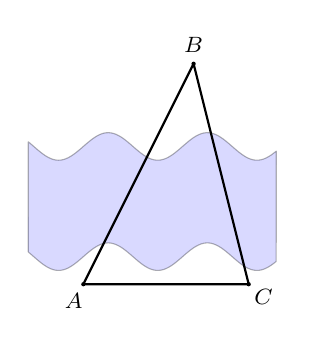
\begin{tikzpicture}[scale=.7, font=\footnotesize, line join=round, line cap=round,>=stealth]
		\path
		(0,0) coordinate (A)
		(2,4) coordinate (B)
		(3,0) coordinate (C)
		;
		\draw [fill=white!50!blue, opacity=0.3, smooth, samples=100, domain=-1:3.5] plot(\x, {sin(\x*200)*0.25+0.5}) -- plot[domain=3.5:-1] (\x, {sin(\x*200)*0.25+2.5}) -- cycle;
		\draw[thick] (B)--(A)--(C)--(B)   ;
		\foreach \x/\g in {A/-120,B/90,C/-40}
		\fill[black] (\x) circle(1.1pt) + (\g:3.5mm) node {$\x$};
	\end{tikzpicture}
	}
\loigiai{
	Ta có $\widehat{B} = 180^\circ - 59{,}95^{\circ}- 82{,}15^{\circ} = 37{,}9^{\circ}$. \\
	Áp dụng định lí sin ta có
	\[
	\dfrac{AB}{\sin C} = \dfrac{AC}{\sin B} \Rightarrow AB = \dfrac{25\cdot\sin 82{,}15^{\circ} }{\sin 37{,}9^{\circ}} \approx 40{,}3~\mathrm{m}.
	\]
	}
\end{vd}
\begin{vd}%[24-25 Bài giảng K10-K11, Phạm Tuấn]%[0H4H2-1]
	\immini{Cho tứ giác $ACBD$ như hình vẽ dưới. Tính độ dài các đoan thẳng $BD$, $CD$, $AD$.
	\dongcham{8}
	% \choiceTF[t]
	% {\True $\widehat{BDC} =  20^\circ$}
	% {$CD > 2160$ m}
	% {\True $BD>1500$ m}
	% {\True $AD>1200$ m}
	}
	{\begin{tikzpicture}[scale=.7, font=\footnotesize, line join=round, line cap=round, >=stealth]
	\path
	(4,3) coordinate (A)
	(1.99,-1.36) coordinate (B)
	(0,0) coordinate (C)
	(6,0) coordinate (D)
	;
	\draw ($(A)!0.5!(C)$) node[above left]{$1800$ m}  ($(B)!0.5!(C)$) node[below left]{$900$ m} ;
	\draw pic["$34^{\circ}$", draw=black,double, angle eccentricity=1.8, angle radius=0.6cm]{angle=D--C--A};
	\draw pic["$35^{\circ}$", draw=black, angle eccentricity=1.8, angle radius=0.5cm]{angle=B--C--D};
	\draw pic["$125^{\circ}$", draw=black, angle eccentricity=1.4, angle radius=0.4cm]{angle=D--B--C};
	\draw[thick] (A)--(C)--(B)--(D)--(A) (C)--(D)   ;
	\foreach \x/\g in {A/90,B/-90,C/180,D/0}
	\fill[black] (\x) circle(1.1pt) + (\g:3.5mm) node {$\x$};
	\end{tikzpicture}}
\loigiai{
	\begin{itemchoice}
		\itemch Ta có $\widehat{BDC} = 180^\circ - 35^\circ - 125^\circ = 20^\circ$.
		\itemch  Áp dụng định lí sin ta có
		$$\dfrac{CD}{\sin 125^\circ} = \dfrac{900}{\sin 20^\circ} \Rightarrow CD \approx 2155{,}54~\mathrm{m}.$$
		\itemch  Áp dụng định lí sin ta có
		$$\dfrac{BD}{\sin 35^\circ} = \dfrac{900}{\sin 20^\circ} \Rightarrow BD \approx 1509{,}32~\mathrm{m}.$$
		\itemch  Áp dụng định lí cosin cho tam giác $ACD$ ta có
		\[
		AD= \sqrt{1800^2+2155{,}54^2-2 \cdot 1800 \cdot 2155{,}54 \cdot \cos 34^\circ} \approx 1205{,}43~\mathrm{m}.
		\]
	\end{itemchoice}
	}
\end{vd}
\begin{dang}{Các công thức tính diện tích tam giác}
	Cho tam giác $ABC$. Ta kí hiệu
	\immini{\begin{itemize}
			\item $h_a, h_b, h_c$ là độ dài các đường cao lần lượt ứng với các cạnh $BC, CA, AB$.
			\item $R$ là bán kính đường tròn ngoại tiếp tam giác.
			\item $r$ là bán kính đường tròn nội tiếp tam giác.
			\item $p$ là nửa chu vi tam giác.
			\item $S$ là diện tích tam giác.
	\end{itemize}}
	{	\begin{tikzpicture}[scale=.9, font=\footnotesize,line join=round, line cap=round,>=stealth]
			\path
			(0,3) coordinate (A)
			(-1.5,0) coordinate (B)
			(3.5,0) coordinate (C)
			(0,0) coordinate (H);
			\draw (A)--(B)--(C)--cycle
			(A)--(H);
			\foreach \x/\g in {A/90,B/180,C/0,H/-90}\fill (\x) circle (1pt)+(\g:.3) node{$\x$};
			\path
			(A)--(B) node[above, midway]{$c$}
			(A)--(C) node[above, midway]{$b$}
			(B)--(C) node[below, midway]{$a$}
			(A)--(H) node[right, midway]{$h_a$};
	\end{tikzpicture}}
	\noindent
	Ta có các công thức tính diện tích tam giác sau:
	\begin{multicols}{2}
		\begin{enumerate}[1)]
			\item $S = \dfrac{1}{2} a h_a = \dfrac{1}{2} b h_b = \dfrac{1}{2} c h_c$.
			\item $S = \dfrac{1}{2} a b \sin C = \dfrac{1}{2} b c \sin A = \dfrac{1}{2} a c \sin B$.
			\item $S = \dfrac{a b c}{4 R}$.
			\item $S = p r$.
		\end{enumerate}
	\end{multicols}
	\begin{enumerate}[1)]
		\setcounter{enumi}{4}
		\item $S = \sqrt{p(p-a)(p-b)(p-c)}$ (công thức Heron).
	\end{enumerate}
\end{dang}
\begin{vd}%[Tex hoá Tài Liệu 10 Mới, Cao Thành Thái]%[0H2B3-1]
	Cho tam giác $ABC$, biết $a=21$, $b=17$, $c=10$.
	\begin{listEX}[2]
		\item Tính diện tích $S$ của $\triangle ABC$ và chiều cao kẻ từ $A$.
		\item Tính bán kính đường tròn nội tiếp $r$.
	\end{listEX}
	\loigiai
	{
	\begin{enumerate}
		\item Nửa chu vi của tam giác $ABC$ là $p=\dfrac{a+b+c}{2} = \dfrac{21+17+10}{2} = 24$.\\
		Diện tích của tam giác $ABC$ là
		\[S=\sqrt{p(p-a)(p-b)(p-c)} = \sqrt{24(24-21)(24-17)(24-10)} = 84.\]
		Ta có $S=\dfrac{1}{2}ah_a$, suy ra $h_a=\dfrac{2S}{a} = \dfrac{2\cdot 84}{21}=8$.
		\item Ta có $S=pr$, suy ra $r=\dfrac{S}{p} = \dfrac{84}{24}=\dfrac{7}{2}$.
	\end{enumerate}
	}
\end{vd}
\begin{vd}%[Tex hoá Tài Liệu 10 Mới, Cao Thành Thái]%[0H2K3-1]
	Cho tam giác $ABC$, có $\widehat{A}=60^\circ$, $b=20$, $c=25$.
	\begin{enumerate}
		\item Tính diện tích $S$ và chiều cao $h_a$.
		\item Tính bán kính đường tròn ngoại tiếp $R$ và bán kính đường tròn nội tiếp $r$.
	\end{enumerate}
	\loigiai
	{
	\begin{enumerate}
		\item Diện tích của tam giác $ABC$ là $S=\dfrac{1}{2}bc\sin A = \dfrac{1}{2}\cdot 20\cdot 25\cdot \sin 60^\circ = 125\sqrt{3}$.\\
		Áp dụng định lí cosin cho tam giác $ABC$ ta có
		\[a^2=b^2+c^2-2bc\cos A = 20^2+25^2-2\cdot 20\cdot 25\cos 60^\circ = 525.\]
		Suy ra $a=\sqrt{525}=5\sqrt{21}$.\\
		Ta có $S=\dfrac{1}{2}ah_a$, suy ra $h_a=\dfrac{2S}{a} = \dfrac{2\cdot 125\sqrt{3}}{5\sqrt{21}} = \dfrac{50\sqrt{7}}{7}$.
		\item Ta có $S=\dfrac{abc}{4R}$, suy ra $R=\dfrac{abc}{4S} = \dfrac{5\sqrt{21}\cdot 20\cdot 25}{4\cdot 125\sqrt{3}} = 5\sqrt{7}$.\\
		Nửa chu vi của tam giác $ABC$ là $p=\dfrac{a+b+c}{2} = \dfrac{5\sqrt{21}+20+25}{2} = \dfrac{45+5\sqrt{21}}{2}$.\\
		Ta có $S=pr$, suy ra $r=\dfrac{S}{p} = \dfrac{125\sqrt{3}\cdot 2}{45+5\sqrt{21}} = \dfrac{15\sqrt{3}-5\sqrt{7}}{2}$.
	\end{enumerate}
	}
\end{vd}
%%=====Ví dụ 16
\begin{vd}%[0H4H3-1]
	Cho tam giác $ABC$ có $AB=100$, $\widehat{B}=100^{\circ}$ và $\widehat{C}=45^{\circ}$. Tính diện tích tam giác $ABC$.
\loigiai{
	\immini{
	Áp dụng định lý sin trong tam giác $ABC$ ta có
	\begin{eqnarray*}
		\dfrac{AB}{\sin C}	&=&\dfrac{AC}{\sin B}\\
		\Leftrightarrow AC&=& \dfrac{AB \sin B}{\sin C}\\
		\Leftrightarrow AC&=&\dfrac{100 \sin 100^{\circ}}{\sin 45^{\circ}}.
	\end{eqnarray*}
	}{\begin{tikzpicture}[>=stealth,line join=round,line cap=round,font=\footnotesize,scale=1]
	\path
	(-0.7,3) coordinate (A)
	(0,0) coordinate (B)
	(3,0) coordinate (C)
	;
	\draw (A)--(B)--(C)--cycle;
	\foreach \d/\g in {A/90,B/-90,C/-90} \fill (\d)node[shift={(\g:0.3)}]{$\d$} circle(1pt);
	\draw pic["$100^{\circ}$",draw=black, angle eccentricity=2, angle radius=0.4cm]{angle=C--B--A};
	\draw pic["$45^{\circ}$",double,draw=black, angle eccentricity=2, angle radius=0.4cm]{angle=A--C--B};
	\path
	(A)--(B) node[left, midway]{$100$};
	\end{tikzpicture}}
	\noindent
	Lại có $\widehat{A}=180^{\circ}-\widehat{B}-\widehat{C}=180^{\circ}-100^{\circ}-45^{\circ}=35^{\circ}$.\\
	Suy ra $S_{ABC}=\dfrac{1}{2} \cdot AB \cdot AC \cdot \sin A=\dfrac{1}{2} \cdot 100 \cdot \dfrac{100 \sin 100^{\circ}}{\sin 45^{\circ}} \cdot \sin 35^{\circ} \approx 3994{,}18$.
	}
\end{vd}
%%=====Ví dụ 18
%%=====Ví dụ 19
\begin{vd}%[0H4H3-1]
	Cho tứ giác lồi $ABCD$ có các đường chéo $AC=x$, $BD=y$ và góc giữa $AC$ và $BD$ bằng $\alpha$. Gọi $S$ là diện tích của tứ giác $ABCD$.
	\begin{listEX}[2]
		\item Chứng minh $S=\dfrac{1}{2}xy \sin \alpha$.
		\item Nếu $AC\perp BD$ thì $S$ bằng bao nhiêu?
	\end{listEX}
\loigiai{
	\immini{
	\begin{enumerate}
		\item
		Ta có $S_{ABCD}=S_{ABD}+S_{CBD}$.\\
		Vẽ $AH$ và $CK$ vuông góc với $BD$. Gọi $I$ là giao điểm của hai đường chéo $AC$ và $BD$.\\
		Ta có $AH=AI \cdot\sin \alpha$, $CK=CI \cdot\sin \alpha$.\\
		\allowdisplaybreaks
		\begin{eqnarray*}
			S_{ABCD}&=&\dfrac{1}{2}AH \cdot BD+\dfrac{1}{2}CK \cdot BD\\
			&=&\dfrac{1}{2} BD(AH+CK)\\
			&=&\dfrac{1}{2} BD(AI+CI) \sin \alpha \\
			&=&\dfrac{1}{2} \cdot BD \cdot AC \sin \alpha\\
			&=&\dfrac{1}{2}\cdot x \cdot y \sin \alpha.
		\end{eqnarray*}
		\item Nếu $AC \parallel BD$ thì $\alpha = 90^{\circ}$.\\
		Suy ra $S=\dfrac{1}{2}xy \sin \alpha=\dfrac{1}{2}xy \sin 90^{\circ} = \dfrac{1}{2}xy$.
	\end{enumerate}
	}{
	\begin{tikzpicture}[scale=1, font=\footnotesize, line join=round, line cap=round,>=stealth]
		\coordinate (O) at (1,1);
		\coordinate (A) at ($(O)+(133:2.5)$) ;
		\coordinate (B) at ($(O)+(198:2.5)$) ;
		\coordinate (C) at ($(O)+(282:2.5)$) ;
		\coordinate (D) at ($(O)+(0:2.5)$) ;
		\coordinate[label=left:$ $] (I) at (intersection cs:first line={(A)--(C)}, second line={(B)--(D)});
		\coordinate (H) at ($(B)!(A)!(D)$);
		\coordinate (K) at ($(B)!(C)!(D)$);
		\draw pic[draw,angle radius=0.2cm]{right angle=A--H--B};
		\draw pic[draw,angle radius=0.2cm]{right angle=D--K--C};
		\draw (A)--(B)--(C)--(D)--(A)--(C) (B)--(D) (A)--(H) (C)--(K);
		\path
		($(A)!0.4!(C)$) coordinate (x)
		($(B)!0.5!(D)$) coordinate (y)
		($(A)!0.6!(C)$) coordinate (x')
		;
		\draw pic[draw=black, angle eccentricity=2.2, angle radius=0.3cm]{angle=C--I--D};
		\fill (x') node[shift={(0:0.3)}]{$\alpha$};
		\foreach \x/\g in {A/130,B/200,C/-90,D/0,H/-90,K/40}
		\fill[black] (\x) circle (1.1pt)+(\g:3mm) node {$\x$};
		\fill (x) node[shift={(0:0.3)}]{$x$};
		\fill (y) node[shift={(90:0.3)}]{$y$};
	\end{tikzpicture}
	}
	}
\end{vd}
\begin{dang}{Giải tam giác}
	Giải tam giác là tính các cạnh và các góc còn lại của tam giác.
\end{dang}
\begin{vd}%[0H2B3-1]
	Giải tam giác $ABC$ biết $b=32$, $c=45$ và $\widehat{A}=87^\circ$.
\loigiai{
	Áp dụng định lí cosin, ta có
	\[a^2=b^2+c^2-2bc \cos A = 32^2+45^2-2\cdot 32 \cdot 45 \cdot \cos 87^\circ=2898 \Rightarrow a \approx 54.\]
	Áp dụng định lí sin, ta có
	\[\dfrac{a}{\sin A}=\dfrac{b}{\sin B}\Rightarrow \sin B =\dfrac{b \sin A}{a}=\dfrac{32\cdot \sin 87^\circ}{54}\approx 0{,}59\Rightarrow \widehat{B} \approx 36^\circ.\]
	Trong tam giác $ABC$ có
	\[\widehat{C}=180^\circ -\left(\widehat{A}+\widehat{B}\right)\approx180^\circ -\left(87^\circ + 36^\circ\right)=57^\circ.\]
	}
\end{vd}
\begin{vd}%[0H2B3-1]
	Giải tam giác $ABC$ biết $\widehat{A}=60^\circ$, $\widehat{B}=40^\circ$ và $c=14$.
\loigiai{
	Trong tam giác $ABC$ có
	\[\widehat{C}=180^\circ -\left(\widehat{A}+\widehat{B}\right)=180^\circ -\left(60^\circ + 40^\circ\right)=80^\circ.\]
	Áp dụng định lí sin, ta có
	\[\dfrac{a}{\sin A}=\dfrac{b}{\sin B}=\dfrac{c}{\sin C}\Rightarrow \heva{&a = \dfrac{c\sin A}{\sin C}=\dfrac{14 \sin 60^\circ}{\sin 80^\circ} \approx 12{,}3\\
	&b = \dfrac{c\sin B}{\sin C}=\dfrac{14 \sin 40^\circ}{\sin 80^\circ} \approx 9{,}1.}\]
	}
\end{vd}
\begin{vd}%[0C4K2-1]%[TeX hóa Sex CD]%[Huỳnh Xuân Tín]
	Cho tam giác $A B C$ có $AB=8$, $AC=7$, $\widehat{ABH}=60^\circ$. Tính độ dài cạnh $B C$ và số đo các góc $A, C$.
\loigiai{
	Đặt $B C=x(x>0)$.\\
	Áp dụng định lí cosin cho tam giác $A B C$ ta có
	\begin{eqnarray*}
		&&A C^2=A B^2+B C^2-2 A B \cdot B C \cdot \cos B \\
		&\Rightarrow& 7^2=8^2+x^2-2 \cdot 8 \cdot x \cdot \cos 60^{\circ} \\
		&\Rightarrow& x^2-8 x+15=0\\
		&\Rightarrow& x=3\text{ hoặc }x=5.
	\end{eqnarray*}
	Vậy $B C=3$ hoặc $B C=5$.\\
	Trường hợp 1: $B C=3$.\\
	Áp dụng định lí sin ta có $\dfrac{B C}{\sin A}=\dfrac{A C}{\sin B}$.\\
	Suy ra $\sin A=\dfrac{B C \sin B}{A C}=\dfrac{3 \sin 60^{\circ}}{7}=\dfrac{3 \sqrt{3}}{14}$.\\
	Do đó, $\hat{A} \approx 21{,}8^{\circ}$ và $\widehat{C} \approx 180^{\circ}-60^{\circ}-21{,}8^{\circ}=98{,}2^{\circ}$.\\
	Trường hợp 2: $B C=5$.\\
	Áp dụng định lí sin ta có $\dfrac{B C}{\sin A}=\dfrac{A C}{\sin B}$.\\
	Suy ra $\sin A=\dfrac{B C \sin B}{A C}=\dfrac{5 \sin 60^{\circ}}{7}=\dfrac{5 \sqrt{3}}{14}$. \\
	Do đó, $\hat{A} \approx 38{,}2^{\circ}$ và $\widehat{C} \approx 180^{\circ}-60^{\circ}-38{,}2^{\circ}=81{,}8^{\circ}$.
	}
\end{vd}
\begin{dang}{Ứng dụng thực tế}%Dạng 5
\end{dang}
\begin{vd}%[Tex hóa THPT]%[Phạm Tuấn]%[0H4H2-1]
	Hai tàu đánh cá cùng xuất phát từ bến $A$ và đi thẳng đều về hai vùng biển khác nhau, theo hai hướng tạo với nhau góc $75^{\circ}$. Tàu thứ nhất chạy với độ $8$ hải lí một giờ và tàu thứ hai chạy với tốc độ $12$ hải lí một giờ. Sau $1{,}5$ giờ thì khoảng cách giữa hai tàu là bao nhiêu hải lí?
\loigiai{
	\immini{
	Gọi vị trí tàu thứ nhất và tàu thứ hai sau khi đi được $1{,}5$ giờ lần lượt là $B$ và $C$. \\
	Ta có $AB=1{,}5 \cdot 8 =12$, $AC=1{,}5 \cdot 12 =18$. \\
	Áp dụng định lí cosin ta có
	\begin{align*}
		BC = \sqrt{12^2+18^2-2 \cdot 12 \cdot 18 \cdot \cos 75^{\circ}} \approx 18{,}9 ~(\text{hải lí}).
	\end{align*}
	Vậy sau $1{,}5$ giờ thì khoảng cách giữa hai tàu là khoảng $18{,}9$ hải lí.
	}
	{
	\begin{tikzpicture}[scale=1, font=\footnotesize, line join=round, line cap=round,>=stealth]
		\path
		(0,0) coordinate (A)
		(75:3) coordinate (B)
		(4,0) coordinate (C)
		;
		\draw pic["$75^{\circ}$", draw=black, angle eccentricity=1.6, angle radius=0.5cm]{angle=C--A--B};
		\draw[thick] (B)--(A)--(C)   ;
		\draw[thick,dashed] (B)--(C) ;
		\foreach \x/\g in {A/-120,B/90,C/-40}
		\fill[black] (\x) circle(1.1pt) + (\g:3.5mm) node {$\x$};
	\end{tikzpicture}
	}
	}
\end{vd}
\begin{vd}%[0H4V3-2]
	\immini{Giả sử $CD=h$ là chiều cao của tháp trong đó $C$ là chân tháp. Chọn hai điểm $A$, $B$ trên mặt đất sao cho ba điểm $A$, $B$, $C$ thẳng hàng. Ta đo được $AB=21$ m, $\widehat{CAD}=65^\circ$, $\widehat{CBD}=43^\circ$. Chiều cao $h$ của khối tháp bằng bao nhiêu? (\textit{làm tròn kết quả đến hàng phần mười}).}
	{\begin{tikzpicture}[smooth,scale=.15,line join=round]
	\draw [fill=blue,smooth,line join=round,blue] (-6.14475,0)..controls +(60:.5) and +(120:.5)..(-5.727,0.3825)..controls +(60:.5) and +(120:.5)..(-4.1775,0.9825)..controls +(60:.5) and +(120:.5)..(-3.0275,2)..controls +(60:.5) and +(120:.5)..(-2.,2.)--(-1.8575,4.5325)--(-1.6275,3.1825)..controls +(70:1) and +(-110:1)..(1.8,5.5825)--(2.,2.)..controls +(60:.5) and +(120:.5)..(2.9225,1.9325)..controls +(60:.5) and +(120:.5)..(4.2225,1.0825)..controls +(60:.5) and +(120:.5)..(5.9225,0.4325)..controls +(60:.5) and +(120:.5)..(6.7725,0)--cycle;
	\draw [fill=blue,smooth,blue] (-1.77,5.8825)--(-1.62,8.7325)..controls +(70:1) and +(-110:1)..(1.48,10.8325)--(1.612,8.0825)..controls +(-110:1) and +(70:1)..(-1.77,5.8825);
	\draw [fill=blue,blue] (-1.45,11.4325)--(-1.22,15) arc (180:0:{1.22} and {.5})--(1.22,15)--(1.34,13.3325)..controls +(-110:1) and +(70:1)..(-1.45,11.4325);
	\draw [line width=.1cm,blue] (-1.18,15)--(-1.22,15.6) arc (180:0:{1.22} and {.5})--(1.22,15.6)--(1.18,15);
	\draw[fill=blue,blue] (0,14) ellipse ({2} and {.5});
	\draw[fill=blue,blue] (0,17.5) ellipse ({.2} and {.8});
	\draw [fill=blue,blue] (0,16.4) circle (.35);
	\draw[fill=blue,blue] (-.9,17) arc (180:0:{.9 and .9});
	\draw [line width=.08cm,blue] (0.87,15)--(0.87,16);
	\draw [line width=.08cm,blue] (-0.87,15)--(-0.87,16);
	\draw [line width=.08cm,blue] (0.33,15)--(0.33,16.1);
	\draw [line width=.08cm,blue] (-0.33,15)--(-0.33,16.1);
	\draw [line width=.06cm,blue] (0.81,16)--(0.81,17.2);
	\draw [line width=.06cm,blue] (-0.81,16)--(-0.81,17.2);
	\path
	(-1,5.3) coordinate (C)
	(.8,11.5) coordinate (D)
	(-14,0) coordinate (A);
	\draw[fill=blue,blue] ($(C)+(60:.6)$)--($(C)+(120:.6)$)--($(C)+(-120:.6)$)--($(C)+(-60:.6)$)--cycle;
	\draw[fill=blue,blue] ($(D)+(60:.6)$)--($(D)+(120:.6)$)--($(D)+(-120:.6)$)--($(D)+(-60:.6)$)--cycle;
	%\draw[yellow](-2,2)--(-1.22,15.9)--(1.22,15.9)--(2,2)--cycle;
	\draw (0,0) node[below]{$C$};
	\draw (-14,0) node[below]{$A$};
	\draw (-20,0)node[left]{$B$}--(5,0);
	\draw (0,0)--(0,18)node[above]{$D$}--(-20,0);
	\draw (0,18)--(-14,0);
	\draw ($(C)!0.2!(D)$) node[right,scale=1]{$h$};
	\draw (-20,0) node[shift={(22:0.70)},scale=.6]{$43^\circ$};
	\draw (-14,0) node[shift={(22:0.70)},scale=.6]{$65^\circ$};
	\draw (-17,0) node[below,scale=0.6]{$21\,$m};
	\path
	(-20,0) coordinate (X)
	(0,18) coordinate (Z)
	(0,0) coordinate (Y)
	(-14,0) coordinate (W);
	\pic [draw=blue,double,angle radius=4mm] {angle=Y--X--Z};
	\pic [draw=blue,,angle radius=4mm] {angle=Y--W--Z};
	\end{tikzpicture}}
	\shortans[0]{$35{,}5$}
\loigiai{
	Ta có $\widehat{CAD}=65^\circ \Rightarrow \widehat{BAD}=115^\circ \Rightarrow \widehat{ADB}=180^\circ-\left(115^\circ+43^0 \right)=22^\circ$.\\
	Áp dụng định lý sin trong tam giác $ABD$ ta có \[\dfrac{AB}{\sin \widehat{ADB}}=\dfrac{BD}{\sin \widehat{BAD}} \Rightarrow BD=\dfrac{AB\cdot \sin \widehat{BAD}}{\sin \widehat{ADB}}.\]
	Tam giác $BCD$ vuông tại $C$ nên có $\sin \widehat{CBD}=\dfrac{CD}{BD} \Rightarrow CD=BD\cdot\sin \widehat{CBD}$.\\
	Vậy chiều cao của tháp là \[CD=\dfrac{AB\cdot\sin \widehat{BAD}\cdot\sin \widehat{CBD}}{\sin \widehat{ADB}}=\dfrac{21\cdot\sin 115^\circ\cdot\sin 43^\circ}{\sin 22^\circ}=34{,}65\,\mathrm{m}.\]
	}
\end{vd}
\begin{vd}%[Dự án Bài giảng K10-11, Phan Văn Thành]%[0H4H3-2]
	\immini{
	Từ một vị trí quan sát $A$, một người nhìn đỉnh $B$ và chân $C$ của nhà cao tầng với các góc tương ứng là $43^{\circ}$ và $16^{\circ}$ so với phương nằm ngang. Biết chiều cao của tòa nhà là $18$ m, tính khoảng cách từ $A$ đến $C$ (\textit{làm tròn kết quả đến hàng phần mười}).
	\choice
	{$13,5\mathrm{~m}$}
	{$14\mathrm{~m}$}
	{\True $15,4\mathrm{~m}$}
	{$15,5\mathrm{~m}$}
	}
	{
	\begin{tikzpicture}[scale=0.6,>=stealth, font=\footnotesize, line join=round, line cap=round]
		\path
		(0,0) coordinate (A)
		(4,3) coordinate (B)
		(4,-1) coordinate (C)
		(4,0) coordinate (H)
		;
		\draw[pattern=bricks,pattern color=brown] (B)--(6,3)--(6,-1)--(4,-1)--(B);
		\foreach \i in {2,3,4,5}
		\draw[fill=white] ({4+1/3},{-1+(2/3)*(\i-1)})--({4+1/3},{-1+(2/3)*(\i-1)+0.5})--({4+2/3},{-1+(2/3)*(\i-1)+0.5})--({4+2/3},{-1+(2/3)*(\i-1)})--cycle
		({5+1/3},{-1+(2/3)*(\i-1)})--({5+1/3},{-1+(2/3)*(\i-1)+0.5})--({5+2/3},{-1+(2/3)*(\i-1)+0.5})--({5+2/3},{-1+(2/3)*(\i-1)})--cycle;
		\draw[dashed](A)--(B)  (A)--(C) (A)--(H);
		\draw pic["$43^{\circ}$", draw=black, angle eccentricity=1.4, angle radius=0.9cm]{angle=H--A--B};
		\draw pic["$16^{\circ}$", draw=black,double, angle eccentricity=1.5, angle radius=1.2cm]{angle=C--A--H};
		\foreach \x/\g in {A/180,B/90,C/140,H/145}
		\fill[black] (\x) circle (1pt)+(\g:3mm) node {$\x$};
		\clip (-0.5,{-1-0.25}) rectangle (6.6,-1) ;
		\draw[fill=gray!30] (-0.5,-1)--(6.6,-1)--(6.6,{-1-0.25})--(-0.5,{-1-0.25})--cycle;
		\foreach \i in {1,2,...,35}
		\draw ({-0.5+0.2*(\i)},-1)--($({-0.5+0.2*(\i)},-1)+(-120:0.3)$) ;
	\end{tikzpicture}
	}
\loigiai{
	Ta có $AH = BH\cdot \cot \widehat{BAH} = CH\cdot  \cot \widehat{CAH}$. \\
	Suy ra
	\begin{eqnarray*}
		&&(BC-CH)\cdot  \cot \widehat{BAH} = CH \cot \widehat{CAH}\\
		&\Leftrightarrow & CH = \dfrac{BC \cdot \cot \widehat{BAH}}{\cot \widehat{CAH}  + \cot \widehat{BAH} } \\
		&\Leftrightarrow & CH =  \dfrac{18 \cdot \cot 43^\circ}{ \cot 16^\circ + \cot 43^\circ}.
	\end{eqnarray*}
	Khoảng cách từ $A$ đến $C$ là
	\[ AC =\dfrac{CH}{\sin 16^\circ} = \dfrac{18\cdot \cot 43^\circ}{ (\cot 16^\circ+ \cot 43^\circ)\sin 16^\circ} \approx 15{,}4\mathrm{~m}.\]
	}
\end{vd}
\subsection{BÀI TẬP RÈN LUYỆN}
%-------------Trắc nghiệm nhiều lựa chọn
\ind{PHẦN I.} \inden{Câu trắc nghiệm nhiều phương án lựa chọn. Mỗi câu hỏi học sinh chỉ chọn một phương án.}
\setcounter{ex}{0}
\Opensolutionfile{ans}[ans/ans-c3b6-lc]
\begin{ex}%[0H4N2-1]
	Cho tam giác $ABC$ có $BC=a$, $CA=b$, $AB=c$. Mệnh đề nào dưới đây đúng?
	\choice
	{$b^2=a^2+c^2$}
	{$a^2=b^2+c^2+2 b c \cdot \cos A$}
	{$\dfrac{a}
	{\cos A}=\dfrac{b}{\cos B}=\dfrac{c}{\cos C}$}
	{\True$c^2=a^2+b^2-2 a b \cdot \cos C$}
\loigiai{
	Mệnh đề đúng là $c^2=a^2+b^2-2 a b \cdot \cos C$.
	}
\end{ex}
\begin{ex}%[Đỗ Minh Phúc]%[0H4N2-1]
	Tam giác $ABC$ có $AB=2$, $AC=1$ và $\widehat{A}=60^{\circ}$. Tính độ dài cạnh $BC$.
	\choice
	{$BC=1$}
	{$BC=2$}
	{$BC=\sqrt{2}$}
	{\True $BC=\sqrt{3}$}
\loigiai{
	Áp dụng định lý cosin ta có
	$$BC^2=AB^2+AC^2-2\cdot AB\cdot AC\cdot \cos\widehat{A}=2^2+1^2-2\cdot 2\cdot 1\cdot\cos 60^\circ=3\Rightarrow BC=\sqrt{3}.$$
	}
\end{ex}
\begin{ex}%[Đỗ Minh Phúc]%[0H4H2-1]
	Tam giác ${ABC}$ có $AB=5$, $BC=7$, $CA=8$. Số đo góc $A$ bằng
	\choice
	{$30^{\circ}$}
	{$45^{\circ}$}
	{\True $60^{\circ}$}
	{$90^{\circ}$}
\loigiai{
	Áp dụng định lý cosin ta có
	$$\cos\widehat{A}=\dfrac{AB^2+AC^2-BC^2}{2\cdot AB\cdot AC}=\dfrac{5^2+8^2-7^2}{2\cdot 5\cdot 8}=\dfrac{1}{2}\Rightarrow\widehat{A}=60^\circ.$$
	}
\end{ex}
\begin{ex}%[Đỗ Minh Phúc]%[0H4H2-1]
	Tam giác $ABC$ có $\widehat{B}=60^{\circ}$, $\widehat{C}=45^{\circ}$ và $AB=5$. Tính độ dài cạnh $AC$.
	\choice
	{\True $AC=\dfrac{5 \sqrt{6}}
	{2}$}
	{$AC=5 \sqrt{3}$}
	{$AC=5 \sqrt{2}$}
	{$AC=10$}
\loigiai{
	Áp dụng định lý sin ta có
	$$\dfrac{AB}{\sin C}=\dfrac{AC}{\sin B}\Rightarrow AC=\dfrac{AB\cdot\sin B}{\sin C}=\dfrac{5\sin 60^{\circ}}{\sin 45^{\circ}}=\dfrac{5 \sqrt{6}}{2}.$$
	}
\end{ex}
\begin{ex}%[Đỗ Minh Phúc]%[0H4N2-1]
	Tam giác $ABC$ có $BC=10$ và $\widehat{A}=30^{\circ}$. Tính bán kính $R$ của đường tròn ngoại tiếp tam giác $ABC$.
	\choice
	{$R=5$}
	{\True $R=10$}
	{$R=\dfrac{10}
	{\sqrt{3}}$}
	{$R=10 \sqrt{3}$}
\loigiai{
	Áp dụng định lý sin ta có
	$$\dfrac{BC}{\sin A}=2R\Rightarrow R=\dfrac{BC}{2\sin A}=\dfrac{10}{2\sin 30^{\circ}}=10.$$
	}
\end{ex}
\begin{ex}%Trắc nghiệm câu 7  Bài 2%[Hoàng Khắc Ngân]%[0H4H2-1]
	Tam giác $ABC$ có $AB=3$, $AC=6$ và $\widehat{A}=60^{\circ} $. Tính bán kính $R$ của đường tròn ngoại tiếp tam giác $ABC$.
	\choice
	{\True $R=3$}
	{$R=3\sqrt{3}$}
	{$R=\sqrt{3}$}
	{$R=6$}
	\loigiai
	{Ta có $BC^2=AB^2+AC^2-2\cdot AB \cdot AC \cdot \cos A = 9+36- 2\cdot 3 \cdot 6 \cdot \dfrac{1}{2}=27$, suy ra $BC=3\sqrt{3}$.\\
	Khi đó $R=\dfrac{BC}{2\cdot \sin A}=\dfrac{3\sqrt{3}}{2\cdot \sin 60^{\circ}}=3$.}
\end{ex}
\begin{ex}%[Lê Hồng Phi, Tex hóa tài liệu 10 mới,2023]%[0H4N2-2]
	Tam giác $ABC$ có $AB=3$, $AC=6$, $\widehat{BAC}=60^{\circ}$. Tính diện tích tam giác $ABC$.
	\choice
	{$S_{\triangle ABC}=9\sqrt{3}$}
	{\True $S_{\triangle ABC}=\dfrac{9\sqrt{3}}
	{2}$}
	{$S_{\triangle ABC}=9$}
	{$S_{\triangle ABC}=\dfrac{9}{2}$}
\loigiai{
	Diện tích tam giác $ABC$ là $$S_{ABC}=\dfrac{1}{2}\cdot AB\cdot AC\cdot\sin\widehat{BAC}=\dfrac{1}{2}\cdot 3\cdot 6\cdot\sin 60^\circ=\dfrac{9\sqrt{3}}{2}.$$
	}
\end{ex}
\begin{ex}%[Lê Hồng Phi, Tex hóa tài liệu 10 mới,2023]%[0H4H2-2]
	Tam giác $ABC$ có $a=21$, $b=17$, $c=10$. Diện tích của tam giác $ABC$ bằng
	\choice
	{$S_{\triangle ABC}=16$}
	{$S_{\triangle ABC}=48$}
	{$S_{\triangle ABC}=24$}
	{\True $S_{\triangle ABC}=84$}
\loigiai{
	Nửa chu vi tam giác là $p=\dfrac{a+b+c}{2}=\dfrac{21+17+10}{2}=24$.\\
	Diện tích tam giác $ABC$ tính theo công thức Heron là
	\begin{eqnarray*}
		S_{\triangle ABC}&=&\sqrt{p(p-a)(p-b)(p-c)}\\
		&=&\sqrt{24\cdot (24-21)\cdot (24-17)\cdot (24-10)}=84.
	\end{eqnarray*}
	}
\end{ex}
\begin{ex}%Trắc nghiệm câu 8 Bài 2%[Hoàng Khắc Ngân]%[0H4H2-2]
	Tam giác $ABC$ có $BC=21$ cm, $CA=17$ cm, $AB=10$ cm. Tính bán kính $R$ của đường tròn ngoại tiếp tam giác $ABC$.
	\choice
	{\True $R=\dfrac{85}
	{2}$ cm}
	{$R=\dfrac{7}
	{4}$ cm}
	{$R=\dfrac{85}{8}$ cm}
	{$R=\dfrac{7}{2}$ cm}
	\loigiai
	{Ta có $p=\dfrac{a+b+c}{2} =24$ và $$S=\sqrt{p(p-a)(p-b)(p-c)}=\sqrt{24\cdot (24-21)\cdot (24-17)\cdot (24-10)} =84\text{ cm}^2.$$
	Khi đó $R=\dfrac{abc}{4S}=\dfrac{21\cdot 17\cdot 10}{4\cdot 84}=\dfrac{85}{2}=42{,}5$ cm.
	}
\end{ex}
\begin{ex}%[Lê Hồng Phi, Tex hóa tài liệu 10 mới,2023]%[0H4H2-2]
	Tam giác $ABC$ có $AB=3$, $AC=6$, $\widehat{BAC}=60^{\circ}$. Tính độ dài đường cao $h_a$ của tam giác.
	\choice
	{$h_a=3\sqrt{3}$}
	{$h_a=\sqrt{3}$}
	{\True $h_a=3$}
	{$h_a=\dfrac{3}{2}$}
\loigiai{
	Diện tích tam giác $ABC$ là $S_{ABC}=\dfrac{1}{2}\cdot AB\cdot AC\cdot\sin\widehat{BAC}=\dfrac{1}{2}\cdot 3\cdot 6\cdot\sin 60^\circ=\dfrac{9\sqrt{3}}{2}$.\\
	Ta có \begin{eqnarray*}
	BC&=&\sqrt{AB^2+AC^2-2\cdot AB\cdot AC\cdot\cos\widehat{BAC}}\\
	&=&\sqrt{3^2+6^2-2\cdot 3\cdot 6\cdot\cos 60^\circ}=3\sqrt{3}.
	\end{eqnarray*}
	Đường cao $h_a$ là $h_a=\dfrac{2S_{\triangle ABC}}{BC}=\dfrac{2\cdot\dfrac{9\sqrt{3}}{2}}{3\sqrt{3}}=3$.
	}
\end{ex}
\begin{ex}%[Nguyễn Tiến]%[0H4H2-2]%Câu 20
	Tam giác $ABC$ có $AB=8$ cm, $AC=18$ cm và có diện tích bằng $64$ cm$^2$. Giá trị của $\sin A$ bằng
	\choice
	{$\sin A=\dfrac{\sqrt{3}}
	{2}$}
	{$\sin A=\dfrac{3}
	{8}$}
	{$\sin A=\dfrac{4}{5}$}
	{\True $\sin A=\dfrac{8}{9}$}
	\loigiai
	{
	Diện tích $\triangle ABC$ là
	\allowdisplaybreaks
	\begin{eqnarray*}
		& & S=\dfrac{1}{2}AB\cdot AC\cdot \sin A\\
		&\Leftrightarrow & \sin A=\dfrac{2S}{AB\cdot AC}=\dfrac{2\cdot 64}{8\cdot 18}=\dfrac{8}{9}.
	\end{eqnarray*}
	}
\end{ex}
\begin{ex}%Câu 23%[Đỗ Đường Hiếu]%[0H4H2-2]
	Tam giác $ABC$ có $AB=5$, $AC=8$ và $\widehat{BAC}=60^\circ$. Tính bán kính $r$ của đường tròn nội tiếp tam giác đã cho.
	\choice
	{$r=1$}
	{$r=2$}
	{\True $r=\sqrt{3}$}
	{$r=2\sqrt{3}$}
\loigiai{
	Ta có $BC^2=AB^2+AC^2-2AB\cdot AC\cdot \cos\widehat{BAC}=5^2+8^2-2\cdot 5\cdot 8\cdot \cos 60^\circ=49$. Suy ra $BC=7$.\\
	Diện tích tam giác $ABC$ là
	$$S=\dfrac{1}{2}AB\cdot AC\cdot\sin \widehat{BAC}=\dfrac{1}{2}\cdot 5\cdot 8\cdot \sin 60^\circ=10\sqrt{3}.$$
	Bán kính $r$ của đường tròn nội tiếp tam giác đã cho là
	$$r=\dfrac{2S}{AB+BC+AC}=\dfrac{2\cdot 10\sqrt{3}}{5+8+7}=\sqrt{3}.$$
	}
\end{ex}
\Closesolutionfile{ans}
\indapan{6}{ans/ans-c3b6-lc}
%---------------------Trắc nghiệm đúng sai
\ind{PHẦN II.} \inden{Câu trắc nghiệm đúng sai. Trong mỗi ý a), b), c), d) ở mỗi câu, học sinh chọn đúng hoặc sai.}
\setcounter{ex}{0}
\Opensolutionfile{ans}[ans/ans-c3b6-ds]
\begin{ex}%[10-11EX-GK1-M25-2425, Đình Nguyên, Đề GK1 trường THPT Phan Chu Trinh, Phú Yên]%[0H4H3-1]
	Tam giác $ABC$ có $\widehat{A}=45^\circ$, $\widehat{B}=15^\circ$, $BC=2$.
	\choiceTF
	{\True $\widehat{C}=120^\circ$}
	{\True Bán kính đường tròn ngoại tiếp tam giác $ABC$ là $R=\sqrt2$}
	{\True Độ dài cạnh $AB$ bằng $\sqrt{6}$}
	{Diện tích tam giác $ABC$ là $\dfrac{3+\sqrt{3}}{2}$}
\loigiai{
	\begin{itemchoice}
		\itemch Ta có $\widehat C=180^\circ-\widehat A-\widehat B=180^\circ-45^\circ-15^\circ=120^\circ$.
		\itemch Ta có $\dfrac{BC}{\sin A}=2R$. Suy ra $2R=\dfrac{2}{\sin 45^\circ}=2\sqrt2$. Do đó $R=\sqrt2$.
		\itemch Ta có $\dfrac{BC}{\sin A}=\dfrac{AB}{\sin C} \Rightarrow AB=\dfrac{BC\cdot \sin C}{\sin A}=\dfrac{2\sin 120^\circ}{\sin 45^\circ}=\sqrt6$.
		\itemch Ta có $\mathrm S_{ABC}=\dfrac{1}{2}BC\cdot AB\cdot\sin B=\dfrac{1}{2}\cdot2\cdot \sqrt{6}\sin 15^\circ=\dfrac{3-\sqrt3}{2}$.
	\end{itemchoice}
	}
\end{ex}
\begin{ex}%[0-HK1-KN-9-ChuongMyB-HaNoi-2324]%[VN-MT-6,Nguyễn Tuấn]%[0H4H3-1]
	Tam giác $ABC$ có $AB=3$, $AC=6$, $\widehat{A}=60^{\circ}$.
	\choiceTF
	{Diện tích tam giác $ABC$ bằng $9\sqrt{3}$}
	{Bán kính $R$ của đường tròn ngoại tiếp tam giác $ABC$ bằng $3\sqrt{3}$}
	{\True Độ dài đường cao kẻ từ $A$ của tam giác $h_a=3$}
	{Tam giác $ABC$ vuông tại $A$}
\loigiai{
	\begin{itemchoice}
		\itemch
		Ta có $S_{\triangle ABC}=\dfrac{1}{2}\cdot AB \cdot AC\cdot\sin\widehat{A}=\dfrac{1}{2}\cdot 3\cdot 6 \cdot\sin 60^{\circ}=\dfrac{9\sqrt{3}}{2}$.
		\itemch
		Theo định lý cosin, ta có
		\begin{eqnarray*}
			BC^2&=&AB^2+AC^2-2AB\cdot AC\cdot \cos A\\
			&=&3^2+6^2-2\cdot 3\cdot 6\cdot \cos 60^\circ\\
			&=&27.
		\end{eqnarray*}
		$\Rightarrow BC=\sqrt{27}=3\sqrt{3}$.\\
		Theo định lý sin ta có
		\[\dfrac{BC}{\sin A}=2R\Rightarrow R=\dfrac{BC}{2\sin 60^\circ}=\dfrac{3\sqrt{3}}{2\cdot\dfrac{\sqrt{3}}{2}}=3. \]
		\itemch
		Áp dụng định lí cosin, ta có
		\[BC^{2}=AB^{2}+AC^{2}-2 AB \cdot AC\cdot \cos A=27 \Rightarrow BC=3\sqrt{3}.\]
		Ta có $S_{\triangle ABC}=\dfrac{1}{2} \cdot A B \cdot A C \cdot \sin \widehat{A}=\dfrac{1}{2} \cdot 3 \cdot 6 \cdot \sin 60^{\circ}=\dfrac{9 \sqrt{3}}{2}$.\\
		Lại có $S_{\triangle ABC}=\dfrac{1}{2}\cdot BC\cdot h_a \Rightarrow h_a=\dfrac{2S}{BC}=3$.
		\itemch
		Ta có $R=\dfrac{1}{2}AC$ nên tam giác $ABC$ vuông tại $B$.
	\end{itemchoice}
	}
\end{ex}
\begin{ex}%[GK1 Việt Đức - Đề 2]%[Lê Minh An]%[0H4V3-2]
	Hai tàu đánh cá xuất phát từ cảng $A$ lúc $8$ giờ, tàu thứ nhất đi theo hướng $S 70^{\circ} E$ với vận tốc $50$ km/giờ. Tàu thứ hai đi theo hướng $N 40^{\circ} E$ với vận tốc $55$ km/giờ. Đi được $75$ phút thì động cơ của tàu thứ nhất bị hỏng nên tàu trôi tự do theo hướng nam với vận tốc $7$ km/giờ. Sau $1$ giờ $30$ phút kể từ khi động cơ bị hỏng, tàu đó neo đậu được vào một hòn đảo C (như hình vẽ).
	\begin{center}
		\begin{tikzpicture}[scale=1, font=\footnotesize, line join=round, >=stealth]
			% Tạo hệ trục tọa độ
			\draw[<->] (-4,0) -- (4,0) node[right] {E};
			\draw[<->] (0,-3) -- (0,3) node[above] {N};
			\node[below] at (0,-3) {S};
			\node[left] at (-4,0) {W};
			% Vẽ điểm A và các điểm khác bằng cách tính tọa độ
			\coordinate (A) at (0,0);
			\coordinate (B) at ({2*sin(70)},{-2*cos(70)}); % Góc 70 độ và độ dài bất kỳ
			\coordinate (x) at ({3*sin(70)},{-3*cos(70)}); % hướng 1
			\coordinate (C) at ($(B)+(0,-1)$); % Từ B di chuyển theo hướng Nam
			\coordinate (D) at ({3*sin(40)},{3*cos(40)});   % Góc 40 độ và độ dài bất kỳ
			\coordinate (y) at ({4*sin(40)},{4*cos(40)});   % hướng 2
			% Vẽ các đoạn thẳng và đường nét đứt
			\draw (D)--(A) -- (B) -- (C);
			\draw[->,dashed] (B) -- (x);
			\draw[->,dashed] (D) -- (y);
			% Ghi nhãn các điểm
			\foreach \x/\g in{A/-150,B/90,C/-90,D/-60}\fill[black](\x) circle (1pt)($(\x)+(\g:3mm)$)node{$\x$};
			% Vẽ và ghi nhãn các góc
			\node at (0.35,-0.4) {$70^\circ$};
			\node at (0.4,0.9) {$40^\circ$};
			% Ghi nhãn hướng
			\node[right] at (y) {$N40^\circ E$};
			\node[right] at (x) {$S70^\circ E$};
		\end{tikzpicture}
	\end{center}
	Gọi $B$ là nơi tàu thứ nhất bị hỏng, $D$ là vị trí của tàu thứ hai tại thời điểm tàu thứ nhất bị hỏng.
	\choiceTF{Quãng đường mà tàu thứ hai đi được sau $75$ phút kể từ khi xuất phát là $62{,}5$ km}
	{\True Lúc $9$ giờ $15$ phút, tàu thứ nhất và tàu thứ hai tạo với cảng $A$ một góc bằng $70^{\circ}$}
	{Lúc $10$ giờ $45$ phút, tàu thứ nhất cách vị trí xuất phát khoảng $59{,}7$ km}
	{\True Hướng từ cảng $A$ tới đảo nơi tàu thứ nhất neo đậu là $S 61{,}5^{\circ} E$}
\loigiai{
	\begin{itemchoice}
		\itemch Đổi $75$ phút $=1{,}25$ giờ. Quãng đường tàu thứ hai đi được là $AD=1{,}25\cdot 55=68{,}75$ (km).
		\itemch Lúc $9$ giờ $15$ phút, tàu thứ nhất và tàu thứ hai tạo với cảng $A$ một góc là $\widehat{DAB}=180^\circ-40^\circ-70^\circ=70^\circ$.
		\itemch
		Ta có $BC\parallel AS$ nên $\widehat{ABC}=180^\circ-70^\circ=110^\circ$.\\
		$AB=50\cdot 1{,}25=62{,}5$ (km).\\
		$BC=7\cdot 1{,}5=10{,}5$ (km).\\
		Lúc $10$ giờ $45$ phút, tàu thứ nhất cách vị trí xuất phát một đoạn là\\
		$AC=\sqrt{AB^2+BC^2-2\cdot AB\cdot BC\cdot \cos 110^\circ}\approx 66{,}8$ (km).
		\itemch Theo định lí sin ta có
		$$\dfrac{BC}{\sin\widehat{BAC}}=\dfrac{AC}{\sin\widehat{ABC}}\Leftrightarrow \dfrac{10{,}5}{\sin\widehat{BAC}}=\dfrac{66{,}8}{\sin 110^\circ}\Rightarrow \sin\widehat{BAC}\approx 0{,}15\Rightarrow \widehat{BAC}\approx 8{,}5^\circ.$$
		Khi đó $AC$ tạo với hướng đi từ A đến hướng Nam một góc khoảng bằng $70^\circ-8{,}5^\circ=61{,}5^\circ$.\\
		Vậy hướng từ cảng $A$ tới đảo nơi tàu thứ nhất neo đậu là $S 61{,}5^{\circ} E$
	\end{itemchoice}
	}
\end{ex}
\begin{ex}%[10-11-12EX-HK1-2425]%[Hữu Bình]%[0H4V3-2]%Câu 13
	\immini{
	Lúc $6$ giờ $30$ phút sáng, bạn An đi xe đạp từ nhà (điểm $A$) đên trường (điểm $B$) phải leo lên và xuống một con dốc (đỉnh dốc $C$) (tham khảo hình bên). Cho biết đoạn thẳng $AB$ dài $656$ m, $\widehat{A}=5^{\circ}$, $\widehat{B}=2^{\circ}$.
	}{
	\begin{tikzpicture}[line join=round, line cap=round]
		\coordinate (A) at (0,0);
		\coordinate (B) at (6,0);
		\coordinate (C) at (2.3,0.8);
		\draw(A)--(B)--(C)--cycle;
		\foreach \i/\g in {A/90,B/90,C/90}{\draw[fill=white](\i) circle (1.5pt) ($(\i)+(\g:3mm)$) node[scale=1]{$\i$};}
	\end{tikzpicture}
	}
	\choiceTF
	{\True Góc $\widehat{ACB}=173^\circ$}
	{\True Quảng đường bạn An đạp xe lên dốc là $187{,}9$ m \textit{(kết quả làm tròn ở hàng phần chục)}}
	{\True Chiều cao $h$ của con dốc theo đơn vi mét \textit{(kết quả làm tròn đến hàng đơn vị)} là $16$ m}
	{Biết rằng tốc độ trung bình lên dốc là $8$ km/h và tốc độ trung bình khi xuống dốc là $23$ km/h. Bạn An đến trường lúc $6$ giờ $38$ phút \textit{(làm tròn đến đơn vị phút)}}
\loigiai{
	\immini{
	\begin{enumerate}
		\item Góc $\widehat{ACB}=180^\circ-2^\circ-5^\circ=173^\circ$.
		\item Áp dụng định lí sin ta có $\dfrac{AC}{\sin B}=\dfrac{AB}{\sin C}$\\
		$\Rightarrow AC=\dfrac{AB\cdot \sin B}{\sin C}=\dfrac{656\cdot \sin 2^\circ}{\sin173^\circ}\approx187{,}9$ m.
		\item $h=CH=AC\sin A\approx187{,}9\cdot \sin 5^\circ\approx 16$ m.
		\item Áp dụng định lí sin ta có $\dfrac{BC}{\sin B}=\dfrac{AB}{\sin C}$\\
		$\Rightarrow BC=\dfrac{AB\cdot \sin B}{\sin C}=\dfrac{656\cdot \sin 5^\circ}{\sin 173^\circ}\approx469{,}1$ m.\\
		Đổi $AC\approx0{,}1879$ km và $CB\approx 0{,}4691$ km.\\
		Tổng thời gian đi qua dốc là $\dfrac{AC}{8}+\dfrac{CB}{23}\approx 0{,}044$ giờ $\approx 3$ phút.\\
		Vậy An đến trường lúc $6$ giờ $33$ phút.
	\end{enumerate}
	}{
	\begin{tikzpicture}[line join=round, line cap=round]
		\coordinate (A) at (0,0);
		\coordinate (B) at (6,0);
		\coordinate (C) at (2.3,0.8);
		\coordinate (H) at (2.3,0);
		\draw(A)--(B)--(C)--cycle;
		\draw(H)--(C);
		\foreach \i/\g in {A/90,B/90,C/90,H/-90}{\draw[fill=white](\i) circle (1.5pt) ($(\i)+(\g:3mm)$) node[scale=1]{$\i$};}
	\end{tikzpicture}
	}
	}
\end{ex}
\Closesolutionfile{ans}
\indapan{3}{ans/ans-c3b6-ds}
%---------------Trắc nghiệm trả lời ngắn
\ind{PHẦN III.} \inden{Câu trả lời ngắn.}
\setcounter{ex}{0}
\Opensolutionfile{ans}[ans/ans-c3b6-kq]
\begin{ex}%[Dự án GKI-10-11]%[Nguyễn Vương Hiển]%[0H4H2-1]
	Cho tam giác $ABC$, biết $BC=8$, $B=45^{\circ}$, $C=60^{\circ}$. Tính độ dài $AB$ \textit{(kết quả chính xác đến hàng phần trăm)}.
	\shortans[oly]{$6{,}29$}
\loigiai{
	\immini{Ta có $\widehat{A}=180^{\circ}-\widehat{B}-\widehat{C}=75^{\circ}$.\\
	Áp dụng định lý sin ta có
	\[\dfrac{AB}{\sin C}=\dfrac{BC}{\sin A}\Rightarrow AB=\dfrac{BC\sin C}{\sin A}=\dfrac{8\sin 60^{\circ}}{\sin 75^{\circ}}=6{,}29.\]
	}{
	\begin{tikzpicture}[>=stealth,line join=round,line cap=round,font=\footnotesize,scale=0.5]
		\clip (-1,-1) rectangle (7,5);
		\path
		(0,0) coordinate (B)
		(4,4) coordinate (A)
		(6,0) coordinate (C);
		\draw  (A)--(B)--(C)--(A);
		\fill[black] (A) circle (1.5pt) node[above right]{$A$}(C) circle (1.5pt) node[below right]{$C$}(B) circle (1.5pt) node[below left]{$B$};
		\draw (0.5,0.5)node[right]{$45^{\circ}$}(4.3,0.5)node[right]{$60^{\circ}$};
		\draw pic[draw, angle radius = 10pt] {angle =C--B--A};
		\draw pic[draw, angle radius = 10pt] {angle =A--C--B};
	\end{tikzpicture}
	}
	}
\end{ex}
\begin{ex}%[0H4H3-1]
	Cho tam giác $ABC$ có $\widehat B=75^\circ $, $\widehat C=45^\circ $ và $BC=5$. Tính bán kính đường tròn nội tiếp $r$ của tam giác $ABC$ \textit{(làm tròn kết quả đến hàng phần trăm)}.
	\par
	\shortans[oly]{1,35}
\loigiai{
	Áp dụng định lí sin, ta có $\dfrac{AB}{\sin C}=\dfrac{AC}{\sin B}=\dfrac{BC}{\sin A}\\
	\Rightarrow \dfrac{AB}{\sin 45^\circ}=\dfrac{AC}{\sin 75^\circ}=\dfrac{5}{\sin 60^\circ}$\\
	$\Rightarrow AC=\dfrac{5\cdot\sin{75^\circ}}{\sin{60^\circ}}=\dfrac{5\sqrt{6}+15\sqrt{2}}{6}$; $AB=\dfrac{5\cdot \sin{45^\circ}}{\sin{60^\circ}}=\dfrac{5\sqrt 6}{3}$.\\
	Diện tích tam giác $ABC$ là $S=\dfrac{1}{2}\cdot BC\cdot BA\cdot \sin B=\dfrac{1}{2}\cdot 5\cdot \dfrac{5\sqrt 6}{3}\cdot\sin 75^\circ=\dfrac{75+25\sqrt{3}}{12}$.\\
	Ta có $p=\dfrac{AB+BC+AC}{2}=\dfrac{5}{2}+\dfrac{5\sqrt{6}+15\sqrt{2}}{12}+\dfrac{5\sqrt{6}}{6}$.\\
	Suy ra $r=S:p=\left(\dfrac{75+25\sqrt{3}}{12}\right):\left(\dfrac{5}{2}+\dfrac{5\sqrt{6}+15\sqrt{2}}{12}+\dfrac{5\sqrt{6}}{6}\right)\approx 1{,}35$.
	}
\end{ex}
\begin{ex}%[0H4V2-2]
	Cho tam giác $ABC$ có $AC=8$ và có  $\widehat{A}=120^{\circ}$. Trên đoạn $AB$ lấy điểm $M$ sao cho $AM=\dfrac{2}{3} AB$. Biết diện tích tam giác $BMC$ bằng $4\sqrt{3}$. Tính độ dài cạnh $AB$.
	\shortans[oly]{$6$}
\loigiai{
	\immini{Ta có $AM=\dfrac{2}{3} AB\Rightarrow BM=\dfrac{1}{3} AB$.\\
	Từ đó $S_{\triangle BMC}=\dfrac{1}{3} S_{\triangle ABC}=4\sqrt{3} \Rightarrow S_{\triangle ABC}=12\sqrt{3}$.\\
	Áp dụng công thức diện tích ta có
	\begin{eqnarray*}
		S_{\triangle ABC}&=&\dfrac{1}{2} AC\cdot AB\cdot \sin \widehat{BAC}\\
		&=&\dfrac{1}{2} AC\cdot AB\cdot \sin 120^{\circ}\\
		&=&\dfrac{1}{2}\cdot 8\cdot AB\cdot \dfrac{\sqrt{3}}{2}
		=2AB\sqrt{3}.
	\end{eqnarray*}
	Suy ra $2AB\sqrt3=12\sqrt{3}\Rightarrow AB=6$. Vậy độ dài cạnh $AB=6$.}
	{\begin{tikzpicture}
	\def\a{4}
	\path 	(0:0) coordinate (B)
	++(0:\a) coordinate (C)
	++(120:.85*\a) coordinate (A)
	($(A)!2/3!(B)$) coordinate (M);
	\draw	(B)--(A)--(C)--cycle	(C)--(M);
	\foreach \x/\g in {A/90,B/180,C/0,M/150}
	\fill[black] 	(\x) circle (1pt)
	($(\g:3mm)+(\x)$) node {$\x$};
	\end{tikzpicture}}
	}
\end{ex}
\begin{ex}%[10-11EX-GK1-M25-2425, Đình Nguyên, Đề GK1 trường THPT Phan Chu Trinh, Phú Yên]%[0H4V3-2]
	\immini{
	Để xác định chiều cao của một tòa nhà cao tầng, một người đứng tại điểm $ M $, sử dụng giác kế nhìn thấy đỉnh tòa nhà với góc nâng $ \widehat{RQA}=79^\circ $, người đó lùi ra xa một khoảng cách $ LM=40 $ m thì nhìn thấy đỉnh tòa nhà với góc nâng $ \widehat{RPA}=53^\circ $. Tính chiều cao của tòa nhà, biết rằng khoảng cách từ mặt đất đến ống ngắm của giác kế đó là $ PL=QM=1{,}4 $  m. \textit{Làm tròn kết quả đến hàng phần mười của mét.}
	\shortans[oly]{72,9}
	}
	{
	\begin{tikzpicture}[scale=.7, font=\footnotesize, line join=round, line cap=round,>=stealth]
		\path
		(0,0) coordinate (P)
		(4,3) coordinate (A)
		(4,-1) coordinate (O)
		(2.5,0) coordinate (Q)
		(2.5,-1) coordinate (M)
		(0,-1) coordinate (L)
		(4,0) coordinate (R)
		;
		\draw (P)--(A) (A)--(6,3)--(6,-1)--(4,-1)--(A) (-0.5,-1)--(6.6,-1) (Q)--(A)  (Q)--(M) (P)--(L);
		\draw[fill=cyan] (A)--(6,3)--(6,-1)--(4,-1)--(A);
		\foreach \i in {2,3,4,5}
		\draw[fill=white] ({4+1/3},{-1+(2/3)*(\i-1)})--({4+1/3},{-1+(2/3)*(\i-1)+0.5})--({4+2/3},{-1+(2/3)*(\i-1)+0.5})--({4+2/3},{-1+(2/3)*(\i-1)})--cycle
		({5+1/3},{-1+(2/3)*(\i-1)})--({5+1/3},{-1+(2/3)*(\i-1)+0.5})--({5+2/3},{-1+(2/3)*(\i-1)+0.5})--({5+2/3},{-1+(2/3)*(\i-1)})--cycle;
		\draw[dashed]   (P)--(R);
		\draw [<->](P)--(L);
		\draw ($(L)!0.5!(M)$) node[above]{$40 \mathrm{~m}$} ($(P)!0.5!(L)$) node[left]{$1{,}4 \mathrm{~m}$} ;
		\draw pic["$79^{\circ}$", draw=black, angle eccentricity=1.5, angle radius=0.7cm]{angle=R--Q--A};
		\draw pic["$53^{\circ}$", draw=black,double, angle eccentricity=1.5, angle radius=0.7cm]{angle=R--P--A};
		\foreach \x/\g in {P/180,A/140,R/140,Q/-60,L/30,M/30,O/140}
		\fill[black] (\x) circle (1pt)+(\g:3mm) node {$\x$};
		\clip (-0.5,{-1-0.25}) rectangle (6.6,-1) ;
		\draw[fill=gray!30] (-0.5,-1)--(6.6,-1)--(6.6,{-1-0.25})--(-0.5,{-1-0.25})--cycle;
		\foreach \i in {1,2,...,35}
		\draw ({-0.5+0.2*(\i)},-1)--($({-0.5+0.2*(\i)},-1)+(-120:0.3)$) ;
	\end{tikzpicture}
	}
\loigiai{
	Ta có $ \widehat{PAQ}= \widehat{AQR}- \widehat{APR}=79^\circ -53^\circ=26^\circ $.\\
	Áp dụng định lí sin trong tam giác $ APQ $, ta có$$ \dfrac{AQ}{\sin P} = \dfrac{PQ}{\sin A}\Rightarrow  \dfrac{AQ}{\sin 53^\circ}= \dfrac{PQ}{\sin 26^\circ}\Rightarrow AQ=\dfrac{PQ\cdot \sin 53^\circ}{\sin 26^\circ}.$$
	Trong tam giác vuông $ AQR $, ta có
	$$ AR=AQ\cdot \sin 79^\circ=\dfrac{PQ\cdot \sin 53^\circ\cdot \sin 79^\circ}{\sin 26^\circ}= \dfrac{40\cdot \sin 53^\circ\cdot \sin 79^\circ}{\sin 26^\circ}\approx 71{,}5 \text{ m}.$$
	Vậy chiều cao của tòa nhà là $ AO=AR+RO\approx 71{,}5+1{,}4=72{,}9 $ m.
	}
\end{ex}
\begin{ex}%[10-11-12EX-HK1-2425]%[Trần Như Cang]%[0H4V3-2]
	\immini{Trong một cuộc đua thuyền ghe được tổ chức trên sông, có hai ghe $A$ và $B$ ở vị trí như hình vẽ. Điểm $K$ là vị trí khán giả đứng xem và quan sát thấy ghe $A$ và ghe $B$ theo các góc tạo với bờ $IK$ lần lượt là $50^\circ$ và $65^\circ$. Điểm $I$ là đích đến của cuộc đua. Lúc ghe $A$, ghe $B$ và đích $I$ thẳng hàng, từ điểm $I$ quan sát thấy ghe $A$ và ghe $B$ tạo với bờ một góc bằng $60^\circ$. Tính khoảng cách giữa hai ghe thuyền (\textit{làm tròn đến hàng đơn vị của mét}).
	\shortans[oly]{111}
	}
	{
	\begin{tikzpicture}[line join = round, line cap=round,>=stealth,font=\footnotesize,scale=.9]
		\tikzset{nguoicheothuyen/.pic={
		\draw[scale=0.8,xshift=15pt,fill=white]
		(0,0)..controls +(10:1) and +(-170:1).. (6,0)
		(0,0)..controls +(-45:1) and +(-135:1).. (6,0)
		(0,0)..controls +(-75:1) and +(-105:1).. (6,0)
		;
		\begin{scope}[yshift=-3pt]
			\draw[fill=black,line width=1pt,rounded corners=1mm] (3,0)--++(1,0.35)--++(100:0.2)--++(195:0.3)--++(-80	:0.2)
			;
			\draw[fill=black]
			(3.00,0.00)--(3,0.35) -- (3.5,0.15) -- (3,0.5)--(2.95,0.55) ..controls +(40:0.03) and +(-40:0.03) .. (2.95,0.00)
			..controls +(100:0.3) and +(180:0.3) ..  (2.80,0.60)
			-- (2.60,0.55) -- (2.60,0.50) -- (2.30,0.20) -- (2.3,0.20)--(2.6,0.35)--(2.6,0)
			(3.47,0.17) circle(1pt)
			(2.3,0.20)circle(1pt)
			;
			\draw[fill=black]
			(2.5,-0.05) ..controls +(40:0.5) and +(140:0.5) ..  ++(0.6,0)
			..controls +(-140:0.1) and +(-40:0.1) ..  cycle
			;
		\end{scope}
		}}
		\path
		(3,3)pic[scale=0.35,xscale=-1]{nguoicheothuyen}
		(2,2)pic[scale=0.35,xscale=-1]{nguoicheothuyen}
		;
		\path
		(0,0) coordinate (I)
		(4,0) coordinate (K)
		(3,3) coordinate (B)
		($(I)!(K)!(B)$) coordinate (A)
		;
		\draw (I)--(K)--(B)--cycle (K)--(A);
		\draw
		pic[draw,angle radius=6mm] {angle = K--I--B}
		pic[draw,angle radius=6mm] {angle = B--K--A}
		pic[draw,angle radius=8mm] {angle = A--K--I}
		pic[draw,angle radius=9mm] {angle = A--K--I}
		;
		\path
		($(I)+(1,0.35)$) node[]{$60^\circ$}
		($(K)+(-0.65,1)$) node[]{$15^\circ$}
		($(K)+(-1.25,0.25)$) node[]{$50^\circ$}
		;
		\foreach \p/\r in {I/-120,K/-20,B/90,A/120}
		\fill (\p) circle (1.2pt) node[shift={(\r:3mm)}]{$\p$};
		\path ($(I)!0.5!(K)$)node[below]{$380$\,m};
	\end{tikzpicture}
	}
\loigiai{
	Áp dụng định lý sin trong tam giác $IKA$, ta có $\dfrac{IA}{\sin 50^\circ}=\dfrac{IK}{\sin 70^\circ}\Rightarrow IA=\dfrac{IK\sin 50^\circ}{\sin70^\circ}$.\\
	Áp dụng định lý sin trong tam giác $IKB$, ta có $\dfrac{IB}{\sin 65^\circ}=\dfrac{IK}{\sin 55^\circ}\Rightarrow IB=\dfrac{IK\sin 65^\circ}{\sin 55^\circ}$.\\
	Khoảng cách giữa hai ghe thuyền là
	\begin{eqnarray*}
		AB&=&IB-IA\\
		&=&\dfrac{IK\sin{65^\circ}}{\sin{55^\circ}}-\dfrac{IK\sin{50^\circ}}{\sin{70^\circ}}\\
		&=&IK\left( \dfrac{\sin 65^\circ}{\sin 55^\circ}-\dfrac{\sin 50^\circ}{\sin 70^\circ}\right)\\
		&=&380\left( \dfrac{\sin 65^\circ}{\sin 55^\circ}-\dfrac{\sin 50^\circ}{\sin 70^\circ}\right)\\
		&\approx& 111 \text{ m}.
	\end{eqnarray*}
	}
\end{ex}
\begin{ex}%[0H4V3-2]
	\immini{Từ vị trí $A$ người ta quan sát một cây cao.
	Biết $AH=3$ (m), $HB=15$ (m), $\widehat{BAC}=40^\circ$. Khi đó chiều cao của cây là (\textit{làm tròn đến hàng phần chục của mét}).
	\shortans[oly]{12,7}
	}
	{\usetikzlibrary{decorations.pathmorphing,shapes}
	\tikzset{
	treetop/.style = {
	decoration={random steps, segment length=0.4mm},
	decorate
	},
	trunk/.style = {
	decoration={random steps, segment length=2mm, amplitude=0.2mm},
	decorate
	}
	}
	\tikzset{
	man/.pic={%
	\fill [rounded corners=1.5] (0,0.4) -- (0,0.4 -- (0.4,0.5 -- (0.4,0.4) --
	(0.325,0.4) -- (0.325,0.7) -- (0.3,0.7) -- (0.3,0) -- (0.225,0) --
	(0.225,0.4) -- (0.175,0.4) -- (0.175,0) -- (0.1,0) -- (0.1,0.7) --
	(0.075,0.7) -- (0.075,0.4) -- cycle;
	\fill (0.2,0.9) circle (0.1);
	\coordinate (-head) at (0.2,1);
	\coordinate (-foot) at (0.2,0);
	}
	}
	\begin{tikzpicture}[scale=0.7, font=\footnotesize,line join = round, line cap = round, >=stealth]
		\path
		(-4,-2) coordinate (A)
		(0,1.2) coordinate (C)
		(0.2,-2.5) coordinate (T)
		(-4,-2.5) coordinate (H)
		(0,-2.5) coordinate (B)
		;
		%\pic[red] at (-5.3,-2.5) (myman) {man};
		\foreach \w/\f in {0.3/30,0.2/50,0.1/70} {
		\fill [brown!\f!black, trunk] (0,0) ++(-\w/2,0) rectangle +(\w,-2.5);
		}
		\foreach \n/\f in {1.2/40,1/50,0.8/60,0.6/70,0.4/80} {
		\fill [green!\f!black, treetop] ellipse (\n/1.5 and \n);
		}
		\draw (H)--(T) (A)--(H) (A)--(C) (A)--(B);
		\pic[draw,"$40^{\circ}$", angle eccentricity=1.4,angle radius=0.8cm]{angle=B--A--C};
		\pic[draw,"$ $", angle eccentricity=1.4,angle radius=0.7cm]{angle=B--A--C};
		\draw pic[draw, angle radius=2mm]{right angle=B--H--A};
		\path (H)--(B) node[below,midway,sloped]{$15$ m};
		\foreach \x/\g in {A/180,B/-90,C/90,H/-90} \fill[black] (\x)+(\g:.3) node {$\x$};
	\end{tikzpicture}}
\loigiai{
	Vì tam giác $AHB$ vuông tại $H$ nên $AB =\sqrt{AH^2+HB^2}= \sqrt{3^2+15^2}=\sqrt{234}$ m.\\
	Ta có \\
	$\sin \widehat{BAH}=\dfrac{BH}{AB}=\dfrac{15}{\sqrt{234}}\Rightarrow \widehat{BAH}\approx 78{,}6^\circ$\\
	Từ đó suy ra $\widehat{ABC} \approx 78{,}6^\circ$ và $\widehat{ACB} \approx 61{,}4^\circ$.\\
	Áp dụng định lý sin cho tam giác $ABC$ ta có $\dfrac{BC}{\sin A}= \dfrac{AB}{\sin C}$.\\
	Suy ra $BC \approx 12{,}7$ m.
	}
\end{ex}
\Closesolutionfile{ans}
\indapan{4}{ans/ans-c3b6-kq}
%------------------Tự luận
\ind{PHẦN IV.} \inden{Tự luận.}
\setcounter{ex}{0}
\begin{ex}%[Tex hóa THPT]%[Phạm Tuấn]%[0H4H3-1]
	\immini{
	Cho tam giác $ABC$ với $AC=8$, $BC=12$, $\widehat{C}=115^{\circ}$. Tính độ dài cạnh $AB$ và các góc $A$, $B$ của tam giác đó.
	}
	{
	\begin{tikzpicture}[scale=.7, font=\footnotesize, line join=round, line cap=round,>=stealth]
		\path
		(0,0) coordinate (A)
		(1.72,1.48) coordinate (C)
		(5,0) coordinate (B)
		;
		\draw (A)--(B)--(C)--(A) ;
		\draw pic["$115^{\circ}$", draw=black, angle eccentricity=1.4, angle radius=0.5cm]{angle=A--C--B};
		\draw ($(A)!0.5!(C)$) node[above left]{$8$}  ($(B)!0.5!(C)$) node[above right]{$12$} ;
		\foreach \x/\g in {A/-120,B/-40,C/90}
		\fill[black] (\x) circle (1pt)+(\g:3mm) node {$\x$};
	\end{tikzpicture}
	}
\loigiai{
	Áp dụng định lí cosin ta có
	\[
	AB = \sqrt{AC^2+BC^2 -2 AC \cdot BC \cdot \cos C} \approx 17.
	\]
	Áp dụng hệ quả định lí cosin ta có $\cos A = \dfrac{AB^2+AC^2-BC^2}{2AB \cdot AC} \approx 0{,}768$.\\
	Suy ra $\widehat{A} \approx 39{,}8^\circ$.\\
	Suy ra $\widehat{B} = 180^\circ - \widehat{A} -\widehat{C}= 180^\circ - 39{,}8^\circ -115^{\circ} = 25{,}2^\circ$.
	}
\end{ex}
\begin{ex}%[0H4H2-1]
	Cho tam giác $ABC$ có $\widehat{A}=72^{\circ}$, $\widehat{B}=83^{\circ}$, $BC=18$. Tính độ dài các cạnh $AC$, $AB$ và bán kính $R$ của đường tròn ngoại tiếp tam giác đó.
\loigiai{
	Ta có $\widehat{C}=180^\circ-\left(\widehat{A}+\widehat{B}\right)=180^\circ-\left(72^\circ+83^\circ\right)=25^\circ$.\\
	Áp dụng định lý sin trong tam giác $ABC$ ta có
	$$\dfrac{AB}{\sin C}=\dfrac{AC}{\sin B}=\dfrac{BC}{\sin A}=2R\Rightarrow\heva{&AB=\dfrac{BC\cdot \sin C}{\sin A}=\dfrac{18\cdot \sin 25^\circ}{\sin 72^\circ}\approx8\\&AC=\dfrac{BC\cdot \sin B}{\sin A}=\dfrac{18\cdot \sin 83^\circ}{\sin 72^\circ}\approx18{,}79\\&R=\dfrac{BC}{2\sin A}=\dfrac{18}{2\cdot \sin 72^\circ}\approx9{,}46.}$$
	}
\end{ex}
\begin{ex}%[Dự án Bài giảng K10-11, Phan Văn Thành]%[0H4H3-1]
	\immini{
	Cho tam giác $A B C$ có $AB=12$, $AC=9$, $\widehat{A}=60^{\circ}$. $M$ là điểm thuộc cạnh $AB$  sao cho $AM=2BM$. Tính cạnh $CM$ và  góc ${BCM}$ \textit{(làm tròn kết quả đến hàng phần mười)}.
	}
	{
	\begin{tikzpicture}[scale=1, font=\footnotesize, line join=round, line cap=round,>=stealth]
		\path
		(0,0) coordinate (A)
		(4,0) coordinate (B)
		;
		\coordinate (M) at ($(A)!{2/3}!(B)$) ;
		\coordinate (C) at ($(A)+(60:3)$) ;
		\draw (A)--(B)--(C)--(A) (C)--(M)
		pic["$60^{\circ}$", draw=black, angle eccentricity=1.5, angle radius=0.7cm]{angle=B--A--C};
		\foreach \x/\g in {A/-120,B/-60,C/90,M/-90}
		\fill[black] (\x) circle (1pt)+(\g:3mm) node {$\x$};
	\end{tikzpicture}
	}
\loigiai{
	Ta có $AM=2BM \Rightarrow BM = \dfrac{1}{3}AB=4$ và $AM=\dfrac{2}{3}AB=8$. \\
	Áp dụng định lí cosin ta có
	\begin{align*}
		&CM^2=AM^2+AC^2-2AM \cdot AC \cos A =8^2+9^2-2 \cdot 8 \cdot 9 \cos 60^\circ  =  73 \Rightarrow CM=\sqrt{73} \approx 8{,}5; \\
		&BC^2=AB^2+AC^2-2AB \cdot AC \cos A =12^2+9^2-2 \cdot 12 \cdot 9 \cos 60^\circ  =  117\Rightarrow BC=\sqrt{117}.
	\end{align*}
	Áp dụng định lí cosin ta có
	\begin{eqnarray*}
		&&BM^2=CM^2+CB^2-2CM \cdot CB \cos \widehat{BCM}  \\
		&\Leftrightarrow & \cos \widehat{BCM} = \dfrac{CM^2+CB^2- BM^2}{2CM \cdot CB}  \\
		&\Leftrightarrow & \cos \widehat{BCM} = \dfrac{73+117-16}{2 \cdot \sqrt{73} \cdot \sqrt{117}} =  \dfrac{29}{\sqrt{949}}\\
		&\Rightarrow& \widehat{BCM} \approx 19{,}7^\circ.
	\end{eqnarray*}
	}
\end{ex}
\begin{ex}%[0H4H3-2]
	\immini{
	Đứng ở vị trí $A$ trên bờ biển, bạn Nam đo được góc nghiêng so với bờ biển tới vị trí $C$ trên đảo là $30^{\circ}$. Sau đó di chuyển dọc bờ biển đến vị trí $B$ cách $A$ một khoảng $100$ m và đo được góc nghiêng so với bờ biển tới vị trí $C$ đã chọn là $40^{\circ}$. Tính khoảng cách từ vị trí $C$ trên đảo tới bờ biển.}{%%%%%%%BỜ BIỂN%%%%%%%%%
	\begin{tikzpicture}[line join=round, line cap=round,scale=0.9,transform shape]
		\clip (-4,-2.5) rectangle (4,2.5);
		\tikzset{dao/.pic={
		\def\H{
		(-1.34,1.1)
		..controls +(60:.1) and +(-160:0) ..  (-1,1.2)
		..controls +(60:.1) and +(140:0) ..  (-.18,1.29)
		..controls +(10:.06) and +(140:0.27) .. (1.1,1.02)
		..controls +(-40:.1) and +(150:0.2) .. (.55,1)
		..controls +(-140:.3) and +(-45:0.2) .. (-.8,1)
		..controls +(170:.2) and +(-60:0.1) .. cycle
		;}
		\draw \H;
		\fill[green!30] \H;
		}}
		\tikzset{nui/.pic={
		\def\T{ %Trời
		(-3.65,1.75)
		..controls +(60:.05) and +(-160:0) ..  (-3.4,1.8)
		..controls +(45:.1) and +(-150:0) ..  (-3.1,1.78)
		..controls +(45:.1) and +(-150:0) ..  (-2.7,1.75)
		..controls +(60:.1) and +(-160:0) ..  (-2.4,1.8)
		..controls +(60:.1) and +(-160:0) ..  (-1.45,1.74)
		..controls +(60:.1) and +(-160:0) ..  (-.4,1.64)
		..controls +(30:.1) and +(160:0.1) ..  (.98,1.74)
		..controls +(40:.1) and +(130:0.1) ..  (2.2,1.76)
		..controls +(30:.1) and +(150:0.1) ..  (3,1.8)
		..controls +(10:.1) and +(170:0.1) ..  (3.66,1.78)--(3.66,1.95)--(-3.65,1.95)--cycle
		;}
		\draw \T;
		\fill[cyan!30] \T;
		\def\N{
		(-3.65,1.75)
		..controls +(60:.05) and +(-160:0) ..  (-3.4,1.8)
		..controls +(45:.1) and +(-150:0) ..  (-3.1,1.78)
		..controls +(45:.1) and +(-150:0) ..  (-2.7,1.75)
		..controls +(60:.1) and +(-160:0) ..  (-2.4,1.8)
		..controls +(60:.1) and +(-160:0) ..  (-1.45,1.74)
		..controls +(60:.1) and +(-160:0) ..  (-.4,1.64)
		..controls +(30:.1) and +(160:0.1) ..  (.98,1.74)
		..controls +(40:.1) and +(130:0.1) ..  (2.2,1.76)
		..controls +(30:.1) and +(150:0.1) ..  (3,1.8)
		..controls +(10:.1) and +(170:0.1) ..  (3.66,1.78)--(3.66,1.16)
		..controls +(175:.2) and +(20:0) ..  (0,1.5)
		..controls +(20:0) and +(20:.7) ..  (-3.65,1.28)--cycle
		;}
		\draw \N;
		\fill[white] \N;
		}}
		\tikzset{bien/.pic={
		\def\B{
		(3.66,1.16)
		..controls +(175:.2) and +(20:0) ..  (0,1.5)
		..controls +(20:0) and +(20:.7) ..  (-3.65,1.28)--(-3.65,-.65)
		..controls +(15:.2) and +(120:0) .. (0,-.62)
		..controls +(-60:0) and +(-160:0.1) .. (3.66,-.65)--(3.66,1.16)
		;}
		\draw \B;
		\fill[cyan!10!] \B;
		\def\C{ %Cát
		(-3.65,-.65)
		..controls +(15:.2) and +(120:0) .. (0,-.62)
		..controls +(-60:0) and +(-160:0.1) .. (3.66,-.65)--(3.66,-1.9)--(-3.65,-1.9)--cycle
		;}
		\draw \C;
		\fill[brown!20] \C;
		}}
		\tikzset{nguoi/.pic={
		\def\N{
		(-3.04,-.64)--(-3.025,-.6)
		..controls +(90:.1) and +(85:0.06) .. (-3.122,-.59)--(-3.11,-.63)
		..controls +(-160:.07) and +(110:0.05) .. (-3.14,-.81)
		..controls +(-40:.01) and +(60:0) .. (-3.14,-.85)
		..controls +(-120:.07) and +(80:0.05) .. (-3.16,-1.1)
		..controls +(-120:.09) and +(80:0.05) .. (-3.18,-1.28)
		..controls +(-120:.02) and +(170:0.01) .. (-3.165,-1.318)--(-3.1,-1.31)--(-3.1,-1.29)
		..controls +(120:.01) and +(-30:0) .. (-3.135,-1.278)
		..controls +(120:.02) and +(-120:0.04) .. (-3.1,-1.1)
		..controls +(-70:.04) and +(120:0.01) ..(-3.096,-1.14)
		..controls +(-120:.04) and +(120:0.01) ..(-3.09,-1.3)
		..controls +(-120:.02) and +(170:0.02) .. (-3.08,-1.34)--(-2.98,-1.34)
		..controls +(70:.03) and +(-70:0.01) .. (-3.045,-1.296)
		..controls +(110:.04) and +(-70:0.01) .. (-3.03,-1.1)
		..controls +(70:.03) and +(-100:0.01) .. (-3.014,-1.04)--(-3,-1.02)
		..controls +(70:.03) and +(-100:0.01) .. (-3.014,-.85)--(-2.97,-.84)
		..controls +(40:.04) and +(-10:0) .. (-2.98,-.7)
		..controls +(110:.04) and +(-20:0.02) .. (-3.043,-.66)--cycle
		;}
		\draw \N;
		\fill[black!70!] \N;
		\def\Q{ %quần
		(-3.045,-.9)
		..controls +(120:.01) and +(-30:0) .. (-3.04,-1.04)
		-- (-3.1,-1.038)
		..controls +(80:.07) and +(-10:0.01) .. (-3.13,-.94)--(-3.124,-.9)--cycle
		(-3.14,-1.04)--(-3.12,-1.04)
		..controls +(80:.07) and +(-10:0.01) .. (-3.134,-.96)--cycle
		;}
		%\draw \Q;
		\fill[orange] \Q;
		}}
		\path
		(0,0)pic[scale=1]{bien} (0,0)pic[scale=1]{dao}
		(0,0)pic[scale=1]{nui}
		(0,0)pic[scale=1]{nguoi} (-1.1,0)pic[scale=1,rotate=180,yscale=-1]{nguoi}
		;
		\draw[dashed] (1.9,-.6)--(-.1,1.1)--(-3,-.54) (-.1,1.1)--(-.1,-.6);
		\draw (-2.6,-.46)--(-2.45,-.4);%gạch góc
		\draw[<->,red,line width=1] (-3,-.6)--(1.9,-.6);
		\path
		(-0.1,1.1) coordinate (C)
		(1.9,-.6) coordinate (B)
		(-3.1,-.6) coordinate (A);
		\node at (-.5,-.7) [below,scale = 0.8]{$250$ m};
		\node at (0.1,0) [above,scale=0.8]{$d$};
		\node at (-2.1,-.6) [above,scale = 0.8]{$30^\circ$};
		\node at (1.1,-.6) [above,scale = 0.8]{$40^\circ$};
		\node at (0,1) [above left]{\tiny Đảo};
		%góc
		\draw (-2.6,-.3)
		..controls +(-50:.09) and +(60:0.01) .. (-2.5,-.6);
		\draw[scale=1,rotate=180,xscale=.6,yscale=-1] (-2.6,-.3)
		..controls +(-50:.09) and +(60:0.01) .. (-2.5,-.6);
		\foreach \x/\g in {A/90,B/90,C/10} \fill (\x) circle (1pt) +(\g:3mm) node{$\x$};
	\end{tikzpicture}}
\loigiai{
	\immini{Ta có $\widehat{C}=180^\circ-\left(\widehat{A}+\widehat{B}\right)=180^\circ-\left(30^\circ+40^\circ\right)=110^\circ$.\\
	Áp dụng định lý sin trong tam giác $ABC$ ta có
	$$\dfrac{AB}{\sin C}=\dfrac{AC}{\sin B}\Rightarrow AC=\dfrac{AB\cdot \sin B}{\sin C}=\dfrac{100\cdot \sin 40^\circ}{\sin 110^\circ}\approx 68{,}4\text{ (m)}.$$
	Diện tích tam giác $ABC$ là
	$$S_{\triangle ABC}=\dfrac{1}{2}AB\cdot AC\cdot\sin A=\dfrac{1}{2}\cdot 100\cdot 68{,}4\cdot \sin 30^\circ=1710\,\left( \text{m}^2\right).$$
	Khoảng cách từ $C$ đến bờ biển là
	$$CH=\dfrac{2S_{\triangle ABC}}{AB}=\dfrac{2\cdot 1710}{100}=34{,}2\text{ (m)}.$$}{	\begin{tikzpicture}[scale=1.1, font=\footnotesize, line join=round, line cap=round, >=stealth]
	\path (0,0) coordinate (A)
	++(30:3) coordinate (C)
	(A)++(0:4.4) coordinate (B);
	\path coordinate (H) at ($(A)!(C)!(B)$);
	\draw (A)--(B)--(C)--(A) (C)--(H);
	\foreach \x/\g in {A/-90,B/0,C/90,H/-90} \fill (\x) circle (1pt) +(\g:3mm) node{$\x$};
	\draw pic[draw, angle radius = 5pt]{right angle = C--H--A};
	\draw pic["$30^{\circ}$",draw=black, angle eccentricity=2.2, angle radius=0.4cm]{angle=H--A--C};
	\draw pic["$40^{\circ}$",double, draw=black, angle eccentricity=2.1, angle radius=0.4cm]{angle=C--B--H};
	\end{tikzpicture}}
	}
\end{ex}
%%=====Bài tập 8
\begin{ex}%[0H4H3-2]
	\immini{Để tính đường kính và diện tích của một giếng nước cổ có dạng hình tròn, người ta tiến hành đo đạc tại ba vị trí $A$, $B$, $C$ trên thành giếng. Kết quả đo được là $BC=5$ m, $\widehat{BAC}=145^{\circ}$.
	Hỏi diện tích của giếng là bao nhiêu mét vuông?
	}
	{\begin{tikzpicture}[>=stealth,line join=round,line cap=round,font=\footnotesize,scale=.6]
	\path
	(0,0) coordinate (O)
	($(O) + (80:2.5)$) coordinate (A)
	($(O) + (155:2.5)$) coordinate (B)
	($(O) + (25:2.5)$) coordinate (C)
	;
	\draw (A)--(B)--(C)--cycle;
	\draw (O) circle(2.5);
	\foreach \d/\g in {A/90,B/180,C/0} \fill (\d)node[shift={(\g:0.3)}]{$\d$} circle(1pt);
	\path
	(B)--(C) node[below, midway]{$5$ m};
	\draw pic[draw=black, angle eccentricity=2.2, angle radius=0.4cm]{angle=B--A--C};
	\fill (A)node[shift={(-90:0.7)}]{$145^{\circ}$};
	\end{tikzpicture}}
\loigiai{
	Đường kính của giếng nước
	$d=2R=\dfrac{BC}{\sin \widehat{BAC}}=\dfrac{5}{\sin 145^{\circ}} \approx 8{,}72$.\\
	Diện tích của giếng nước
	$S=\pi R^{2}= \pi \dfrac{d^{2}}{4} \approx 59{,}68$ (m$^{2}$).
	}
\end{ex}
\begin{ex}%[0H4V3-2]
	\immini{Bạn $A$ đứng ở đỉnh của tòa nhà và quan sát chiếc diều, nhận thấy góc nâng (góc nghiêng giữa phương từ mắt của bạn $A$ tới chiếc diều và phương nằm ngang) là $\alpha=35^{\circ}$; khoảng cách từ đỉnh tòa nhà tới mắt bạn $A$ là $1{,}5$ m. Cùng lúc đó ở dưới tòa nhà, bạn $B$ cũng quan sát chiếc diều và thấy góc nâng là $\beta=75^{\circ}$; khoảng cách từ mặt đất tới mắt bạn $B$ cũng là $1{,}5$ m. Biết chiều cao tòa nhà là $h=20$ m. Hỏi chiếc diều bay cao bao nhiêu mét so với mặt đất?}{\begin{tikzpicture}[>=stealth,line join=round,line cap=round,font=\footnotesize,scale=0.8]
	\begin{scope}[shift=({0.2,0})]
		% Con dieu
		\filldraw[fill=orange!50,draw=brown] (3.5,5)--(2.8,4.9)--(2.6,5.5)--(3.2,5.6)--cycle;
		\draw[color=brown] (3.5,5)--(2.6,5.5) (2.8,4.9)--(3.2,5.6);
		\draw[line width=0.5mm,rounded corners,color=orange] (3.5,5)--(3.7,5.1)--(4,4.9)--(4.4,5.1) (3.5,5)--(3.6,4.8)--(3.9,4.9)--(4.5,5);
	\end{scope}
	% Cac chi tiet con lai
	\draw (0,0)--(2,0)--(2,4.2)--(0,4.2)--(0,0);
	\draw (1,0)--(1,4.2);
	\foreach \x in {0.7,1.4,...,3.5}{
	\draw (0,\x)--(2,\x);
	}
	\path
	(2,4.55) coordinate (A)
	(3.2,4.55) coordinate (A')
	(2,0.35) coordinate (B)
	(3.2,0.35) coordinate (B')
	(3.2,5.25) coordinate (C)
	;
	\draw (3.2,0)--(2,0)--(A)--(C)--(B);
	\draw[dashed] (C)--(3.2,0) (A)--(A') (B)--(B');
	\foreach \d/\g in {A/180,B/180} \fill (\d)node[shift={(\g:0.3)}]{$\d$} circle(1pt);
	\pic[draw,angle radius=4mm,angle eccentricity=1.5] {angle = A'--A--C};
	\pic[draw,angle radius=4mm,angle eccentricity=1.5] {angle = B'--B--C};
	\pic[draw,angle radius=5mm,angle eccentricity=1.5] {angle = B'--B--C};
	\fill (0,1.4)node[shift={(180:0.3)}]{$h$};
	\fill (A)node[shift={(13:0.65)}]{$\alpha$};
	\fill (B)node[shift={(40:0.75)}]{$\beta$};
	\end{tikzpicture}
	}
\loigiai{
	\immini{
	Ta có $AI$ là khoảng cách từ đỉnh của tòa nhà tới mắt bạn $A$ nên $AI=1{,}5$ m.\\
	$BE$ là khoảng cách từ mặt đất tới mắt của bạn $B$ nên $BE=1{,}5$ m.\\
	Lại có $h=IB+BE \Rightarrow IB=h-BE=20-1{,}5=18{,}5$ (m).\\
	Và $AB=AI+IB=1{,}5+18{,}5=20$ (m).\\
	Ta có $\widehat{CAB}=\alpha+90^{\circ}=35^{\circ}+90^{\circ}=125^{\circ}$;\\ và $\widehat{ABC}=90^{\circ}-\beta=90^{\circ}-75^{\circ}=15^{\circ}$.\\
	Tam giác $ABC$ có $\widehat{ABC}+\widehat{CAB}+\widehat{AC B}=180^{\circ}$ (định lí tổng ba góc trong tam giác).\\
	Suy ra $\widehat{AC B}=180^{\circ}-(\widehat{ABC}+\widehat{CAB})=180^{\circ}-\left(15^{\circ}+125^{\circ}\right)=40^{\circ}$.
	}{
	\begin{tikzpicture}[>=stealth,line join=round,line cap=round,font=\footnotesize,scale=0.8]
		% Cac chi tiet con lai
		\draw (0,0)--(2,0)--(2,4.2)--(0,4.2)--(0,0);
		\draw (1,0)--(1,4.2);
		\foreach \x in {0.7,1.4,...,3.5}{
		\draw (0,\x)--(2,\x);
		}
		\path
		(2,4.55) coordinate (A)
		(3.2,4.55) coordinate (A')
		(2,0.35) coordinate (B)
		(3.2,0.35) coordinate (B')
		(3.2,5.25) coordinate (C)
		;
		\draw (3.2,0)--(2,0)--(A)--(C)--(B);
		\draw[dashed] (C)--(3.2,0) (A)--(A') (B)--(B');
		\foreach \d/\g in {A/180,B/180} \fill (\d)node[shift={(\g:0.3)}]{$\d$} circle(1pt);
		\pic[draw,angle radius=4mm,angle eccentricity=1.5] {angle = A'--A--C};
		\pic[draw,angle radius=4mm,angle eccentricity=1.5] {angle = B'--B--C};
		\pic[draw,angle radius=5mm,angle eccentricity=1.5] {angle = B'--B--C};
		\fill (0,1.4) node[shift={(180:0.3)}]{$h$};
		\fill (A) circle (1.5pt) node[shift={(13:0.65)}]{$\alpha$};
		\fill (B) circle (1.5pt) node[shift={(40:0.75)}]{$\beta$};
		\fill (C) circle (1.5pt) node[shift={(90:0.2)}]{$C$};
		\fill (B') circle (1.5pt) node[shift={(0:0.3)}]{$H$};
		\fill (2,4.2) circle (1.5pt) node[shift={(-45:0.3)}]{$I$};
		\fill (2,0) circle (1.5pt) node[shift={(-90:0.3)}]{$E$};
		\fill (3.2,0) circle (1.5pt) node[shift={(-90:0.3)}]{$K$};
	\end{tikzpicture}
	}
	\noindent
	Áp dụng định lí sin trong tam giác $ABC$ ta có: $\dfrac{AB}{\sin \widehat{AC B}}=\dfrac{BC}{\sin \widehat{CAB}}$.\\
	Do đó $BC=\dfrac{AB \cdot \sin \widehat{CAB}}{\sin \widehat{AC B}}=\dfrac{20 \cdot \sin 125^{\circ}}{\sin 40^{\circ}} \approx 25{,}5$ (m).\\
	Tam giác $CBH$ vuông tại $H$ nên
	$$\sin \widehat{CBH}=\dfrac{C H}{BC} \Rightarrow CH=BC \cdot \sin \beta=25{,}5\cdot \sin 75^{\circ} \approx 24{,}6 \textrm{ (m).}$$
	Lại có $HK=BE=1{,}5 ~m$.\\
	Do đó $CK=CH+HK=24{,}6+1{,}5=26{,}1$ (m).\\
	Vậy chiếc diều bay cao $26{,}1$ m so với mặt đất.
	}
\end{ex}
\Closesolutionfile{ans}